\documentclass[12pt]{amsbook}
\usepackage{amsmath,amssymb,graphicx}
\usepackage{mathpazo}
\usepackage{pdfsync}
\usepackage{listings}
\usepackage{hyperref}
\usepackage{color}
\usepackage[margin=2.25cm]{geometry}
\usepackage[all]{xy}
%\usepackage{draftwatermark}
%\SetWatermarkText{Rough Draft}
%\SetWatermarkScale{1}

% this defines the environment for typesetting bits of code
\lstnewenvironment{code}[0]
{\lstset{
    backgroundcolor=\color{white},
    tabsize=4,
    rulecolor=\color{black},
    language=haskell,
        basicstyle=\Small,
        aboveskip={1.5\baselineskip},
        columns=fixed,
        showstringspaces=false,
        extendedchars=true,
        breaklines=true,
        prebreak = \raisebox{0ex}[0ex][0ex]{\ensuremath{\hookleftarrow}},
        frame=none,
        showtabs=false,
        showspaces=false,
        showstringspaces=false,
        identifierstyle=\color[rgb]{0.0,0.0,0.0},
        keywordstyle=\color[rgb]{0.0,0,0.0},
        commentstyle=\color[rgb]{0,0,0},
        stringstyle=\color[rgb]{0.0,0,0.0},
    upquote=false
}}
{}

\newcommand{\elm}[1]{\texttt{#1}}

\title{Thinking Algebraically with Elm \\ Version 0.81}
\author{\copyright\ 2015-2017, Christopher Kumar Anand}
\date{9 October 2017}

\begin{document}
\maketitle

\vfill
\begin{center}
  This book is dedicated to the student volunteers, teaching assistants and 
  graduate students for helping to reimagine literacy,
  but especially to Curtis d'Alves. 
\end{center}
\vfill
\newpage

\tableofcontents


%\chapter{Changes}\label{Ch:Changes}
%
%- hanoi
%
%- talk about pipelines more, "assembly lines"
%  - move fold into chapter with map
%  ( delete FRP )
%
%- graphicsApp chapter following map
%  - draw a fence
%
%- basement
%
%- notificationsApp chapter follow stateDiagrams
%  - add ELM Architecture
%  
%- complexity (add diagrams?)
%
%- gameApp - pong
%   - slides template
%   
%- algebraic expressions
%
%- CPU


%\chapter*{ToDo}


%https://www.crcpress.com/A-Functional-Start-to-Computing-with-Python/Herman/9781466504554


\chapter*{Preface}
%
This edition of this evolving book has changed its name from ``Thinking Computationally'' to ``Thinking Algebraically''.  
This reflects the coming into focus of why our approach to programming works,
and what we consider to be most important:  giving people tools which (1) connect computing to the mathematics curriculum thereby giving children a better chance of succeeding in Algebra and opening up educational pathways, (2) making learning easier by building in knowledge gained since the 1970s, and (3) starting budding programmers off on a path will lead to high quality software at a time when careless, ignorant and unethical software developers are too often in the headlines. 
Why have we abandoned the more common ``computational thinking''?  
Mostly because it means too many things to different people, including well-intentioned claims which have not been backed up by evidence.

If you already know something about old-fashioned ``real-world'' programming, 
welcome to the future! 

Please send comments and bug-fixes to \verb|anandc@mcmaster.ca|.

\chapter{Tower of Hanoi}

We start with a seemingly simple children's puzzle, but whose solution involves some really powerful aspects of Algebraic Thinking.

In the Tower of Hanoi, your task is to move a tower made by stacking blocks of diminishing size, one on top of another.  You can move one block at a time to one of three bases.  At no time can a larger block rest on a smaller block.  All the blocks have different sizes.

Assuming you are seeing this problem for the first time, the first question is, what questions should you ask yourself?  For which sizes of tower can we solve the problem?  How many moves are required to move the tower with a given number of blocks.

Take some time to think about the problem, and solve it if you can.  If your solution is good, you should have no trouble explaining the solution to a friend.

How did you explain your solution to a friend?  Did you use notation you have used before in algebra or geometry?  Did you make up your own symbolic language?  Could you explain your solution entirely in English?

If your math teachers have done a good job, you started by writing down what you know about the problem, and maybe even assigning variable names.  Here's what I came up with:

\begin{verbatim}
n = number of blocks
{A,B,C} = set of places
{1,2,...n} = the blocks
\end{verbatim}

A surprising feature of this problem, which reflects a general trend in algebraic thinking, is that a seemingly more difficult problem has a simpler solution.  In this case, figuring out how many moves it will take to move a tower of size $n$.  Here is where using algebra, and the Divide \& Conquer principle makes the difference between impossibly convoluted and incredibly simple.  Let $m_n$ be the number of moves required to move a tower of size $n$ from one place to another.  That gives us simple notation.

The DnC principle appeals to a particular kind of teamwork.  It asks us to assume we have friends who will share their solution to a simpler problem so that we can build on that.  In this case, if we are asked to move a tower of size $n$, we can assume that friends have already figured out how to move a tower of size $1$ through $n-1$.  The key is the $n-1$ solution.

Take a few minutes and try to describe a solution to the tower $n$ problem, assuming that you can call on friends to move a tower of size $n-1$.

Well, if friends will move a tower of size $n-1$, they will move the top part of your tower, which is itself a tower of size $n-1$, leaving you to move one block, the one on the bottom, which we will call the $n$th block.  So if you need to move the tower from $A$ to $B$, your job is to move the $n$th block from $A$ to $B$.  To be able to do your job, you need your friends to move the upper $n-1$ blocks from $A$ to $C$ to get them out of the way.  Then you can move your block, after which your friends can move the $n-1$ blocks from $C$ to $B$.  So the number of steps will be

$$
m_n = m_{n-1} + 1 + m_{n-1}
$$

Let's apply this formula to a specific case:

$$
\begin{aligned}
m_3 & = & m_2 + 1 + m_2 \\
    & = & (m_1 + 1 + m_1) + 1 + (m_1 + 1 + m_1) \\
    & = & (1 + 1 + 1) + 1 + (1 + 1 + 1) \\
    & = & 7
\end{aligned}
$$

Now to get 7, we have used the hopefully obvious fact that we can move a tower with 1 block in 1 move.  But there are no obvious facts for computers!  If we had asked a computer to use the definition of $m_n$ in terms of $m_{n-1}$ it would have continued

{\small
$$
\begin{aligned}
m_3 & = & m_2 + 1 + m_2 \\
    & = & (m_1 + 1 + m_1) + 1 + (m_1 + 1 + m_1) \\
    & = & ((m_0 + 1 + m_0) + 1 + (m_0 + 1 + m_0)) + 1 + ((m_0 + 1 + m_0) + 1 + (m_0 + 1 + m_0)) \\
    & = & (((m_{-1} + 1 + m_{-1}) + (m_{-1} + 1 + m_{-1})) + 1 + ((m_{-1} + 1 + m_{-1}) + (m_{-1} + 1 + m_{-1})) ) \\
       & &     + 1 + (((m_{-1} + 1 + m_{-1}) + (m_{-1} + 1 + m_{-1})) + 1 + ((m_{-1} + 1 + m_{-1}) + (m_{-1} + 1 + m_{-1})) ) \\
\end{aligned}
$$
}

and it would have continued to continue until the end of time or it ran out of memory to store the nonsense answer or some physical component failed.

Here is another good lesson about algebraic thinking.  No matter what crazy thing a computer does, people have to take the blame, because people are doing the thinking, coming up with a set of rules and the computer faithfully carries them out.  Until we figure out rules for common sense, computers will not have it, and while that may come sooner than many expect, you can bet it won't come before your next assignment is due---so you figure out the rules.

Philosophical discussions are great, but we still have a problem to solve!  How can we do it?  We need to put in the rule that a person with common sense would have inserted, that 

$$
m_1 = 1
$$
So we could express our procedure as follows:

Given an $m_n$ to calculate, use repeated substitutions to reduce $m_n$ to a number, where we replace
$$
m_1 \text{ with } 1
$$
and for any values of n bigger than 1, we replace
$$
m_n \text{ with } m_{n-1} + 1 + m_{n-1}.
$$
There isn't really any point in writing all of this out, since a person would probably figure that out, but it happens to be very close to how we would use ELM to tell a computer the same thing.

\begin{code}
m n = case n of
        1         -> 1
        otherwise -> m (n-1) + 1 + m (n-1)
\end{code}

Note a few differences between standard algebraic notation and ELM.  Instead of using subscripts to differentiate different values $m_1, m_2, ...$, we use a function \elm{m} depending on an input \elm{n}.  For now, this is just a difference of notation, but functions have the potential to be more general.  The next difference is that we capture all of the substitution rules together by considering all the different cases, using a \elm{case} statement.  This takes up a bit more space on the page in some cases, but it is much clearer if all the rules are together, and the fact that there are multiple rules is signaled by \elm{case} and \elm{of}.  The case statement always works the same way:  The \elm{case} and \elm{of} bracket an expression whose value determines the case.   In this case, the variable \elm{n}.  On the following lines, values line up on the left, separated by \elm{->} (arrows) to the expression used to calculate the function value on the right.  There is one special value, \elm{otherwise}, which catches all the values which do not match any of the other cases.  Finally, unlike in algrebra, multiplication requires a symbol, \elm{*}, and ELM will not accept a definition like \elm{(x+a)(x+b)} in which writing expressions next to each other indicates multiplication, even though this is common in algebra.  One good reason is that ELM allows variable names to be words, rather than single symbols.

You can try this definition for yourself, by typing this text into ***need url for box which captures function definition and tabulates some answers***

*** put in table here ***

At this point we have pointed out the differences, but there are more similarities than differences.  For example, parentheses change the order of operations (which you probably didn't even think about), the operations + and - work as you would expect, and we have variables.  We will talk more about variables, but for now, we'll rely on your understanding of variables from algebra.

One big difference between how we will use ELM and how you have previously used math, is that we just defined our own function \elm{m} on the first day.  Whereas you probably used algebra to solve word problems for years before you learned about a function, maybe it was $\sin(\theta)$ or $\sqrt{x}$, and if you found the concept daunting, then you are not alone.  The funny thing is that you have been using functions most of your life!  Because $+$ is a function.  It takes two numbers and gives you back their sum.  In fact, ELM treats functions like \elm{+} like any other function, and you can even create your own functions written with a symbol or symbols between two input variables.

If you now feel silly for having struggled with the idea of a function, you are not alone, but in fact, there is more we can say about functions besides the fact that they have inputs and outputs, which will make things even clearer.  But first we need to talk about the inputs and outputs, ie the values.  And before that, we better finish our Tower of Hanoi example!

To solve the full problem, we will again use the DnC strategy, so let's spell out the strategy in more detail:  We need to identify three steps:

\begin{itemize}
\item[\textbf{Divide:}]  Within the original problem, identify smaller subproblems of the same type, unless it is small enough to solve immediately.
\item[\textbf{Conquer:}]  Solve the subproblems using the same strategy.
\item[\textbf{Combine:}]  Combine the solutions to the subproblems into a solution to the original problem
\end{itemize}

Sounds simple, but pay close attention to the requirement that the subproblems be of the same type and not subdivide infinitely.  In our first example, the problem was to count the number of moves required to move a tower of size $n$.  All of the problems involve moving a tower, only the size changes, and the towers are readily ranked by size.

Here's an example which fails:  Mow a field by dividing it into two equal pieces and getting two friends to each mow half.  When they are finished, the field is mowed.  The problem:  mow a piece of a field is always the same problem, and if your friends are as lazy as you, they will follow your lead and get two friends to mow halves of their halves.  The problem is that there is no smallest size of field, so nobody would ever get around to doing any mowing.  If we slightly change the problem, and start with a field of 32 hectares, and in the divide step we specify that when the patch to be mowed is 1 hectare, the unlucky friend of a friend will have to go buy a goat and supervise it to insure it munches evenly, then the Divide and Conquer strategy would work.

Here's another way it could fail:  You sneak into the kitchen and steal a gingerbread person, but after escaping detection for a day, you start to worry about potential incarceration, and want to dispose of the body before any detectives come snooping.  So you get some friends and break off the arms, legs and head, and give each friend a piece of anatomy to disappear.  This time you will successfully disappear the evidence, but not using Divide and Conquer, because the subproblems (arms, legs, head, torso) are not the same as the whole person.  You cannot break a leg off an arm, nor an arm off a head.  So what we have is a strategy which disposes of one body, but it won't hide criminality at a large scale, involving, say, boxes of gingerbread people.

Back to the Tower of size $n$:

\begin{itemize}
\item[\textbf{Divide:}]  
The top $n-1$ blocks are a tower in their own right, but smaller by one.  A tower with 1 block cannot be divided, but it can be moved in one step.
\item[\textbf{Conquer:}]  
Calculate the number of steps to move the tower of size $n-1$, call it $m_{n-1}$.
\item[\textbf{Combine:}]  
To move the tower of size $n$, we need to move the smaller tower, move the bottom and move the smaller tower again, so we need $m_{n-1} + 1 + m_{n-1}$ steps.
\end{itemize}
What about moving the tower?  You may have devised your own notation for moves, but some notation is required to avoid writing torturously long sentences in English.

Move Tower of size $n$ from $x$ to $y$ using additional place $z$.
\begin{itemize}
\item[\textbf{Divide:}]  If the tower has size 1, move that piece from $x$ to $y$, which we will write as $(x,y)$, otherwise the top $n-1$ blocks are a smaller tower.
\item[\textbf{Conquer:}]  Apply this procedure to produce a sequence of steps for moving the top tower from $x$ to $z$ using $y$.  Call that sequence $s(x,z,y)$, and apply it again to find a sequence $s(z,y,x)$ to move a tower of size $n-1$ from $z$ to $y$ using $x$.
\item[\textbf{Combine:}]  Join together the two sequences with one additional move:  $s(X,Z,Y)$ followed by $(x,y)$ followed by $s(z,y,x)$.
\end{itemize}
To write this in ELM, we need to define our set of places, which is a distinct type of thing, apart from numbers, letters, words, buffalos, and every other thing we need in our program.  We define a new type of thing like this:

\begin{code}
type Place = A | B | C
\end{code}

The type is obvious.  Giving the new type of thing a name must use a capital letter, hence Place and not place, and the things of that type must also start with capital letters, and are separated by vertical bars.

For two things together, we can use a pair, ie (A,B), in the same way that we use (7,3) for Cartesian coordinates on the plane to group together the horizontal and vertical positions. We can use the pair to represent movements, but if we were already using pairs for other things, we should create a new type for movements to keep things straight.  I'll show you how later.

Since we need many moves, we need a way of putting individual moves together in a finite sequence.  ELM has a List type for this, with two functions we will need a lot:

[x] takes a thing x, and makes a list of length one with it.
xs ++ ys  takes two lists of the same type of thing and joins them together into a bigger list.

With them, we can solve our tower problem:

\begin{code}
move n x y z = case n of
                 1 ->         [(x,y)]
                 otherwise -> (move (n-1) x z y)++[(x,y)]++(move (n-1) z y x) 
\end{code}

Woah!  That was a long chapter, all to explain three lines of ELM!  This is typical of the Divide and Conquer strategy.  Once you figure out how to divide up your problem, it is usually easy to write the code, especially in a language like ELM.  The tricky part is that the divide step is not always obvious.  Let's make sure we remember the three parts:  in the code above, underline the parts which correspond to conquering.

\begin{code}
move n x y z = case n of
                 1 ->         [(x,y)]
                 otherwise -> (move (n-1) x z y)++[(x,y)]++(move (n-1) z y x) 
\end{code}

Now underline the parts corresponding to combining:

\begin{code}
move n x y z = case n of
                 1         -> [(x,y)]
                 otherwise -> (move (n-1) x z y)++[(x,y)]++(move (n-1) z y x) 
\end{code}

\chapter{\texttt{map} and Assembly Lines}

*** put fold here ***

We started this book with Divide \& Conquer because it captures so much of algebraic thinking.
(1) With the right scheme for division,
Divide \& Conquer enables the division of work
among a growing set of computers, 
which is the key to scaling a solution up to 
internet scale.
(2) With the right reformulation, any task a computer can perform, can be expressed as a Divide \& Conquer algorithm.
(3) Even though the individual tasks are simple, Divide \& Conquer procedures can accomplish complex tasks.

But every algorithm is not a Divide \& Conquer algorithm, and confusing different algorithm patterns is a good way to get stuck at the implementation step.
So let's look at some special cases of Divide \& Conquer which are easier to implement directly, starting with \texttt{map}.

When you can divide into \emph{smallest} problems in one step, rather than dividing into \emph{smaller} problems of the same type, you probably want to use map.
The \texttt{map} function applies to collections of data, but let's start with lists, which we have seen before.

\section{Map}
As a simple problem, let's say we have a list like\texttt{[1,2,3,4,5,6,7]} but we want to double each element to make a list of even numbers.  The \texttt{map} function does this
\begin{code}
doubleElements list = map multByTwo list
multByTwo x = 2 * x
\end{code}
computes \textit{[2,4,6,8,10,12,14]}.  Try it yourself on \texttt{http://elm-lang.org/try}.

Although they make nice, short examples, \texttt{map} is not restricted to numbers!  Its type
\begin{code}
map : (a -> b) -> List a -> List b
\end{code}
says that map takes two arguments%
\footnote{Documentation for all of the core packages includes this type information.  
See \texttt{http://package.elm-lang.org/packages/elm-lang/core/2.1.0/List}.
}.  
The first one \texttt{(a -> b)} is a function from 
type \texttt{a} to \texttt{b}.
In our example, both \texttt{a} and \texttt{b} are the type \texttt{Int}, but they could be anything.
They can be anything, but they determine the
types of the input and output lists (and vice versa).
The second argument is a list of type \texttt{a} (\texttt{: List a}) and the output a list of type  
\texttt{b}.
 
Let's look at a practical real-world example. 
First-year students, often living away from home for the first time,
need a lot of advice about things like what can safely go in the dishwasher. 
So we made this handy data type and function.
\begin{code}
type KitchenStuff = Spoon | Plate | Ladle | Microwave | PizzaBox

dishwasherSafe x = case x of
                     Spoon      -> True
                     Plate      -> True
                     Ladle      -> True
                     Microwave  -> False
                     PizzaBox   -> False
\end{code}
But with all the clubs, and the long walk across campus, they do not have time to apply the function to items individually, but with \texttt{map}, then don't have to!
\begin{code}
allSafe = map dishwasherSafe [Spoon,PizzaBox]
\end{code}
gives \texttt{[True,False]}.
So in this case, \texttt{map dishwasherSafe : List KitchenStuff -> List Bool}.

Using \texttt{map} looks powerful, and it is.
Instead of creating a recipe for programmers to implement,
the recipe is captured as function.
This is the common feature of functional programming languages like ELM which are driving their adoption in industry.
You may be aware that the most common languages in industry are object-oriented languages, and have heard of some like Java and C++.
A few decades ago, object-oriented languages offered software architects a way of organizing large pieces of software which, when done right, 
offered much greater flexibility and extensibility than the previous procedural languages.
But over many years, a dark side to these languages emerged.  
Projects often failed to meet their goals, 
and often sinking more money into them hastened their collapse.
Managers were desperate to diagnose failing projects and successful architects wanted to explain why some of their projects succeeded.
The funny thing about software is that after writing a million lines of code, 
you can easily be farther from your destination than when you started,
and to most outsiders, and even many insiders it is hard to tell when this is the case.

Well, a lot was learned by people who wrote a lot of software, and a practical cookbook for successful software design was written.
Called "Design Patterns: Elements of Reusable Object-Oriented Software" by Gamma, Johnson, Vlissides and Booch, it basically said, if you are going to implement a common pattern, do it in a standard way, and name it so developers coming after you know what you are aiming to do.
The standard patterns are called design patterns,
and the book sold over half a million copies,
and most people consider it to be wildly successful.
The weakness of design patterns 
is that they still need to be implemented correctly,
and the languages at the time did very little to help programmers do this.

In contrast, design patterns implemented in functional languages can mostly be implemented as functions themselves,
and often in a couple of lines.
This is possible because functional languages treat functions the same as other variables,
which in Computer Science is the definition of being
``first class''%
\footnote{This is a weird cultural thing in Computer Science, that the default class is first class,
with the assumption that everyone deserves first class treatment, and anything less is implicitly treated as a defect in the system.
Compare this to airlines, where flying first class is  ridiculously expensive and restricted to a privileged few.
}.  
It is still possible to apply higher-order functions like \texttt{map} to the wrong inputs,
but many wrong inputs will be rejected as having incompatible types, 
and the code is short enough to make the pattern and its inputs transparent.
In non-function languages, the pattern implementation is often spread over multiple modules making it difficult to check for consistency.


\medskip
Enough philosophy!  We've seen how simple using  \texttt{map} is. 
But how is it a special case of Divide \& Conquer?
What are the subproblems?  Here they are:
\begin{itemize}
\item[\textbf{Divide:}]  Separate the first element from the rest of the input list.  The rest of the list is still a list, so that's our subproblem.
\item[\textbf{Conquer:}]  Apply this procedure to get a new list whose elements are the result of applying the function argument to the rest of the list.
\item[\textbf{Combine:}]  Take the solution to the subproblem, which is a list, and prepend the result of applying the function argument to the first element.
\end{itemize}
When we implement this in ELM, we also need to take care of the base case, which here is when the list is empty, and so has no first element.
\begin{code}
map fun list = case list of
                 (x :: xs) -> (fun x) :: (map fun xs)
                 []        -> []
\end{code}

\subsection{Anonymous Functions}
%
On its own \texttt{map} is powerful, 
but its usefulness is magnified by being able to 
define simple functions right there in the first \texttt{map} argument, without having to give them a name, and use another line.  Instead of defining
\texttt{multByTwo} above, we could instead use the 
fact that we can use any infix operator like \texttt{+} or \texttt{*}, as a normal function by putting it in parentheses, like so
\begin{code}
multByTwo x = (*) 2 x
\end{code} 
and to save a bit of typing could have used the definition
\begin{code}
multByTwo = (*) 2
\end{code} 
which is called a partial application of the function \texttt{(*)}.
Now, I personally do not recommend using this style a lot, because you it is not visually obvious that \texttt{multByTwo} is a function taking one argument,
but inside a \texttt{map}
\begin{code}
evens n = map ((*) 2) [1..n]
\end{code} 
cannot cause any confusion, and just saved us a line of code.
But it gets better, when we can compose these functions.
In math, functions can be composed with $\circ$, as in
$$
(f \circ g) (x) = f ( g (x) ),
$$
meaning that the function $f\circ g$ takes an input $x$, feeds it to $g$ and feeds that output to $f$ as an input.
In ELM, there are different composition operations
\begin{code}
f <| g x = f (g x) = g x |> f
\end{code}
depending on whether you want outputs to flow left or right into other functions as inputs.
You have probably seen this used to move shapes 
\begin{code}
shape1 = filled red (circle 10) |> move (10,10)
\end{code}
and note that \texttt{move (10,10)} is a partially applied function, since \texttt{move} takes two inputs, but once we give it the first one (the shift vector), 
we have a function with one input, which it gets from
the left of the \texttt{|>}.
So values move across the composition operators in the 
direction of the pointy part.

So ELM notation is more flexible, in allowing both left-to-right and right-to-left compositions,
but this is not quite the same as the $\circ$ composition of mathematical functions.  
The analogues of $\circ$ are \texttt{>>} and \texttt{<<}:
\begin{code}
(f << g) x = f (g x) = (g >> f) x
\end{code} % FIXME these are not ELM =, we should use something else
Which is actually less convenient than the preview composition operators.
In fact, we could insert those operators here as well
\begin{code}
(f << g) x = (f << g) <| x = x |> (f << g) = f (g x)
\end{code}
which is just confusing things,
so what is the point?
The point is that we can compose functions inside \texttt{map}.
So instead of defining a compound function to use in map
\begin{code}
sinePoint x = sin (2 * pi / 10 * x)
hillAndValley = map sinePoint [0..9]
\end{code}
we could use
\begin{code}
hillAndValley = map (sin << ((*) (2*pi/10))) [0..9]
\end{code}
which saves us a line.
Now you may wonder if this is really better, 
since we have so many years of experience looking at expressions more like \texttt{sinePoint},
and you would have a point.
But first of all, this definitely does not apply 
to most cases, e.g., if you need to move and rotate a bunch of shapes
\begin{code}
dancingShapes = map (move (10,10) << rotate (degrees 45)) standingShapes
\end{code}
and secondly, we have another way of putting the $x$ back into anonymous functions,
called a lambda expression
\begin{code}
hillAndValley = map (\ x -> sin(2*pi/10*x)) [0..9]
\end{code}
This looks a bit like a case in a \texttt{case}
expression,
and happily, it means the same thing, except
that there is only one case, and \texttt{x}
input which is mapped to \texttt{sin(2*pi/10*x)}.
They are called lambda expressions 
because the Greek letter $\lambda$ was
used to represent the binding of a variable 
to an expression to define a function,
almost exactly as in ELM,
except that we use \texttt{\symbol{92}} as a discount version of 
$\lambda$, because typing $\lambda$ would be
too time consuming.
Since it was defined by Alonzo Church as a way of
defining computation, 
and proving things about which functions can be computed (which, surprisingly, is not true of all functions),
it was shown to be equivalent to defining
computability in terms of a machine
(specifically a Turing machine, defined by Alan Turing),
and it has become a symbol of computer science.
The place where programming language enthusiasts meet is called \texttt{lambda-the-ultimate.org}, 
and a good place to find out what is cool in programming languages,
and all Computer Science superheros have $\lambda$s stitched into their stretchy suits.

\chapter{To be or not to be in the Basement}
%
Einstein used so-called thought-experiments,
in which he imagined an experiment to evaluate 
the consequences of a theory.
His elevator experiment led to the formulation
of relativity, the most accurate theory we have of gravity.

We're going to do our own elevator experiment, and from it develop a theory for change and a tool for modelling change, called a state diagram.
With state diagrams, we can model changes to physical systems unlucky enough to be connected to our computers and changes to the graphical user interface through which we interact with our users.

You probably remember learning about state in science class.
And if you don't, just shake your head until the generated heat melts those frozen thoughts, and gets them flowing again.
The states of matter look like
\begin{center}
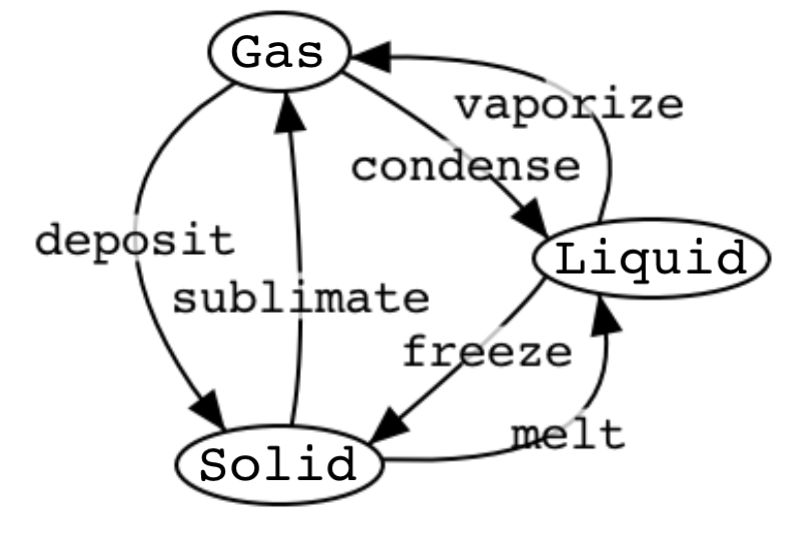
\includegraphics[width=0.4\textwidth]{gasLiquidSolid.png}
\end{center}
where each of the bubbles is a state,
and the arrows are called phase transitions.

In general, when we see a diagram like this in computer science, we call it a graph, the bubbles nodes, and the lines edges.
If the edges have arrows for direction,
it's a directed graph.


\section{State Diagrams}
A State Diagram is directed graph, with nodes we call states, 
and edges we call transitions.
A game graph is very similar to a State Diagram, because there is always a place (state) we are in,
and for this to change, something has to happen.
The real state diagram corresponding to a game would also include any 
items you are carrying, and in some games whether certain mosters are 
dead or not.
This extra information significantly complicates the state diagram,
to the point where nobody could follow it.
Since keeping track of the state of mechanical devices, like elevators,
subway trains, etc., is rather important,
Computer Scientists have developed more complicated versions of state diagrams
called State Charts, which can include nesting (diagrams within diagrams),
and tools to create, visualize and verify charts.
Other tools can even create multiple programs to control the devices and
react to outside events, so that the diagrams themselves play the role of
the program, and the programmer gets to draw pictures instead of write code.

The only thing not normally allowed in a State Diagram is a bi-directional edge.
If the same transition can go in both directions, two arrows are drawn.
While we sometimes do not draw transitions which return to the same state
in order to simplify our diagrams,
it is unusual in state diagrams that each transition only effects one state,
as in the game graph.

State Diagrams, are a graphical representation of Finite State Machines,
which are the usual way of giving Computer Science an a mathematical foundation 
allowing theoretical computer scientists to prove things like
that some programs will go on forever without stopping, 
that one algorithm will take longer to solve a problem than another,
that a the solution produced by an algorithm is correct,
and that the running algorithm always has certain properties (importanly safety properties).

State is always present when software interacts with the real world.

\section{Implementing in ELM}

How do we model state and transitions in ELM?

$$\text{states} = \text{data}$$
$$\text{transitions} = \text{functions}$$
I know that is really complicated, but you just have to memorize it.

In ELM, we can always recognize data types by the \verb|type| keyword,
but forming lists and tuples is another way of creating data.
Be careful when using tuples that the meaning of the data is clear.
Although tuples are really convenient, you probably need a comment explaining
what the different components of the tuple represent,
because you do not have descriptive names the way you do with constructors.

\vspace{-12pt}
\begin{code}
module StateDiagram where
\end{code}

\subsection{Example: an Elevator} 

\emph{State} captures everything we need to know about what is happening \emph{now},
so we know what can happen next, and what actions a user could request.
\begin{itemize}
    \item doors, open and closed
    \item be on a floor or in between floors
    \item doing nothing, or going to a floor
    \item call buttons can be pressed on floors, or in the elevator
\end{itemize}
\emph{Transitions} capture both user requests and actions and processes coming to a completion.
\begin{itemize}
    \item elevator can arrive at a floor
    \item doors can open
    \item doors can close
    \item people can press buttons
    \item elevator arrives at place where button is lit, and button goes dark
    \item door should close if no motion is detected

\end{itemize}
    
\medskip
Data recording the state of the elevator has multiple components.
Let's start small, with recording the state of one door:
\vspace{-12pt}
\begin{code}
type Door = Open | Closed
\end{code}
Two transitions (each function is represented by arrows labelled by function name).
\vspace{-12pt}
\begin{code}
openDoor Open   = Open    -- this is needed in ELM, sometimes omit in diagram
openDoor Closed = Open

closeDoor Open   = Closed
closeDoor Closed = Closed
\end{code}

We can capture these two states and two transitions with a diagram

\begin{center}
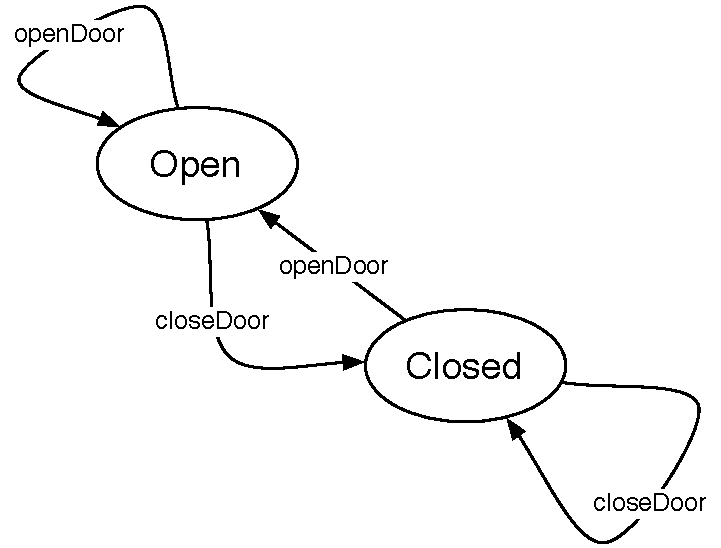
\includegraphics[width=.5\textwidth]{openClose.pdf}
\end{center}
Note again that when things get complicated, 
we often omit transition edges which come back to the same state.

\medskip

Going back to tracking state, we obviously need to know where the 
elevator is.  
There are many ways of doing this, and we came up with
different solutions, but decided to go with
recording the state as being at a floor, or going to a floor.
A more complicated elevator might record the exact position between
floors, 
and if you are going to support smartphones apps which tell you 
when your elevator will arrive, 
you would need to keep track of the speed of the elevator 
and the number of people getting on and off, ...
\vspace{-12pt}
\begin{code}
type Floor = Basement
           | ToBasement 
           | Ground 
           | ToGround
           | First
           | ToFirst
\end{code}

The state of one button:
\vspace{-12pt}
\begin{code}
data Button = LitUp | Dark
\end{code}

Transitions corresponding to buttons being pressed
3 call buttons, these are user-initiated state transitions

Transition functions always have type \verb|State -> State|,
and we can give them all types together.
\vspace{-12pt}
\begin{code}
callToBasement, callToGround, callToFirst, arriveAtGround, arriveAtBasement, arriveAtFirst
  : (Floor,(Button,Button,Button)) -> (Floor,(Button,Button,Button))
\end{code}

Some state transitions are initiated by the user, or by external events.
In this case, the user can call an elevator by pressing a button.
Elevators do not have many external events, but there probably some elevators
out there which detect earthquakes and come to a stop.
\vspace{-12pt}
\begin{code}
callToBasement state = case state of
  (Basement,  (bb,gb,fb))  -> (Basement,  (Dark,Dark,Dark))
  (ToBasement,(bb,gb,fb))  -> (ToBasement,(LitUp,Dark,Dark))
  (Ground,    (bb,gb,fb))  -> (ToBasement,(LitUp,Dark,Dark))
  (First,     (bb,gb,fb))  -> (ToBasement,(LitUp,Dark,Dark))
  (ToGround,  (bb,gb,fb))  -> (ToGround,  (Dark,LitUp,Dark))
  (ToFirst,   (bb,gb,fb))  -> (ToFirst,   (Dark,Dark,LitUp))

callToGround state = case state of
  (Basement,  (bb,gb,fb))  -> (ToGround,  (Dark,LitUp,Dark))
  (ToBasement,(bb,gb,fb))  -> (ToBasement,(LitUp,Dark,Dark))
  (Ground,    (bb,gb,fb))  -> (Ground,    (Dark,Dark,Dark))
  (First,     (bb,gb,fb))  -> (ToGround,  (Dark,LitUp,Dark))
  (ToGround,  (bb,gb,fb))  -> (ToGround,  (Dark,LitUp,Dark))
  (ToFirst,   (bb,gb,fb))  -> (ToFirst,   (Dark,Dark,LitUp))
\end{code}
We leave it as a homework problem to write the \verb|callToFirst| function.

There are also environment-initiated state transitions.
\vspace{-12pt}
\begin{code}
arriveAtGround state = case state of
   (Basement,  (bb,gb,fb))  -> (Ground,    (Dark,Dark,Dark))
     -- this should really cause an error, since we arrived somewhere we were not going
  ++" and got a signal that we arrived on the ground floor"
   (ToBasement,(bb,gb,fb))  -> (ToBasement,(LitUp,Dark,Dark))
   (Ground,    (bb,gb,fb))  -> (Ground,    (Dark,Dark,Dark))
   (First,     (bb,gb,fb))  -> error $ "oops, we think we are on the first floor,"
  ++" and got a signal that we arrived on the ground floor"
   (ToGround,  (bb,gb,fb))  -> (Ground,    (Dark,Dark,Dark))
   (ToFirst,   (bb,gb,fb))  -> (ToFirst,   (Dark,Dark,LitUp))
\end{code}
We leave it as a homework problem to write the 
\verb|arriveAtBasement| and
\verb|arriveAtFirst| functions.
Our best hope of getting all of these cases right is
to \emph{start} with a state diagram,
or in this case, we can simplify things by drawing
separate diagrams for the position of the elevator:
\begin{center}
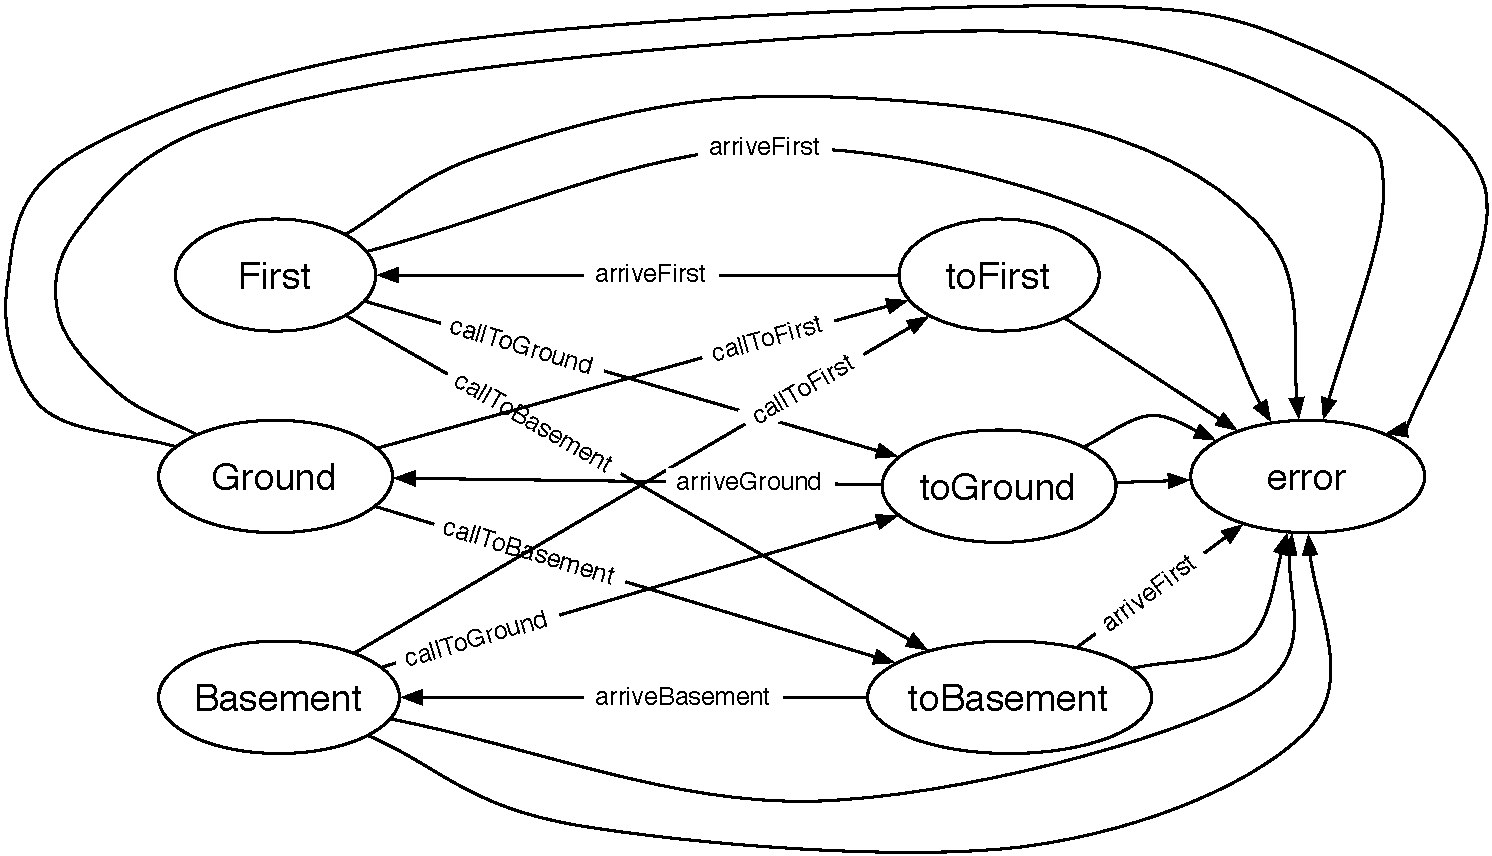
\includegraphics[width=0.75\textwidth]{elevator.pdf}
\end{center}
and the lighting of the buttons:
\begin{center}
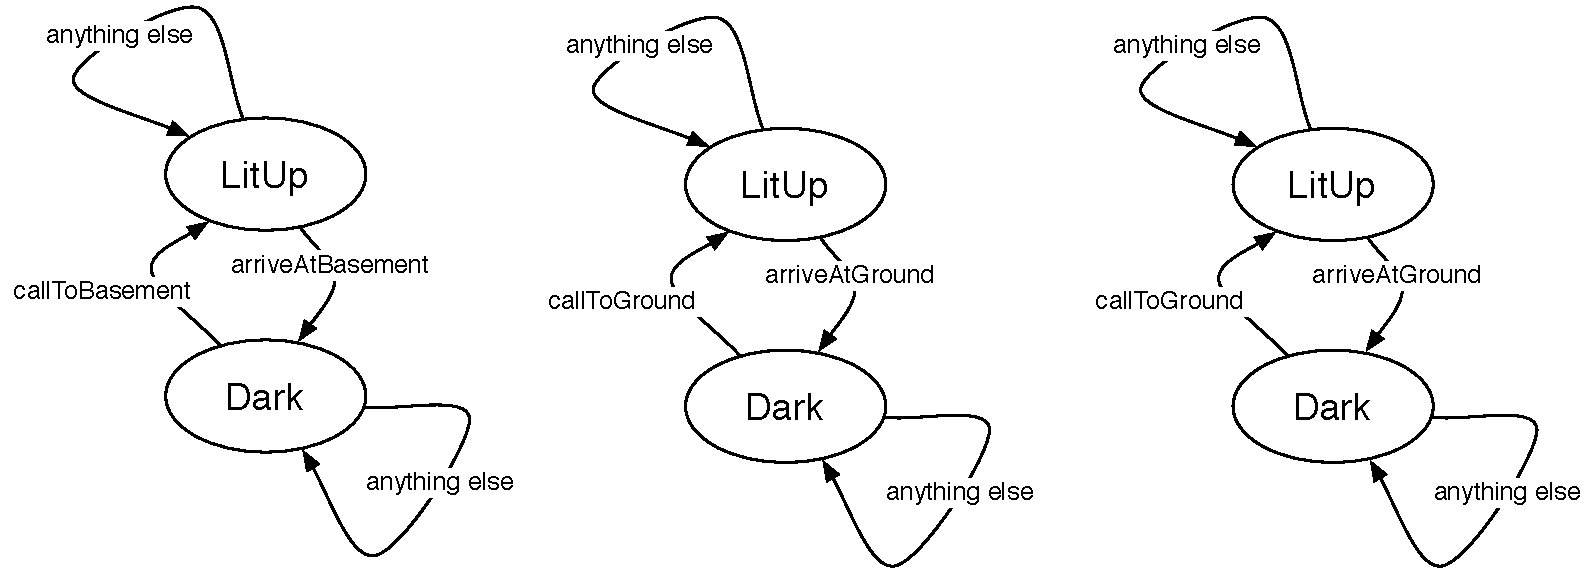
\includegraphics[width=0.75\textwidth]{elevatorButtons.pdf}
\end{center}

But, in our defence, we were still learning about transitions when
we developed this example in class.

\medskip
\emph{Hey!} Why is the state of the door not integrated into the other state?
People are going to get pretty upset when they find out the door doesn't open!
To do this we would need to extend the state, by adding the door state to the 
tuple, or creating a new set of constructors.
This is left as a homework problem.

\section{The StateDiagrams Module}

Let's return to basic science again, and the question that probably bugged you the most:  who drew that masterpiece of a diagram?
ELM, of course!
And for the right price, you can draw your own neat diagrams, all you need is our \texttt{StateDiagrams} module which you import along with the graphics collage to draw it in,
\begin{code}
import StateDiagrams exposing (..)
import Graphics.Collage exposing (..)
\end{code}
then define a type with your favourite states,
\begin{code}
type States = Solid | Liquid | Gas
\end{code}
define the transitions via functions
(which in this case we define to leave all states alone, other than the ones they change),
\begin{code}
melt x = case x of
           Solid -> Liquid
           other -> other
freeze x = case x of
             Liquid -> Solid
             other  -> other
sublimate x = case x of
               Solid -> Gas
               other -> other
deposit x = case x of
              Gas   -> Solid
              other -> other
condense x = case x of
               Gas   -> Liquid
               other -> other
vaporize x = case x of
               Liquid -> Gas
               other  -> other
\end{code}
and use the \texttt{viewStateDiagram}
function to draw it:
\begin{code}
main = collage 400 400 
         [viewStateDiagram [(Solid,(-50,-50))
                           ,(Gas,(-50,50))
                           ,(Liquid,(40,0))
                           ]
                           [(melt,"melt",[(Solid,(20,-40))])
                           ,(freeze,"freeze",[(Liquid,(0,-20))])
                           ,(vaporize,"vaporize",[(Liquid,(20,40))])
                           ,(condense,"condense",[(Gas,(-5,25))])
                           ,(deposit,"deposit",[(Gas,(-85,7))])
                           ,(sublimate,"sublimate",[(Solid,(-45,-7))])
                           ]
                           Nothing
                           Nothing
         ]
\end{code}
This is the hard part, because in addition to
a list of the states you want drawn, you need to figure out Cartesian coordinates to pin them to,
and in addition to the transitions,
you need to decide from which initial states to draw 
them and where to pin the labels.
Note that while the states are data types, 
and ELM just knows how to show them as strings of characters,
transitions are functions which ELM cannot show,
so we need to provide a string to display.

\chapter{Fold, Signals and Functional Reactive Programming}
%
I know you are impatient to learn about creating interactive programs,
and we do have the key concept behind us---State---but we need a bit
more practical knowledge to put this knowledge to use in ELM.

Let's take a look at a simple game, Peekaboo.
We need to import a couple of familiar modules,
and new modules for getting the position of the 
mouse an something called \texttt{Signal}.
\begin{code}
module Peekaboo where
import Graphics.Element exposing (..)
import Graphics.Collage exposing (..)
import Color exposing (..)
import Mouse
import Signal
\end{code}
Next, we have a new type for the main function, \texttt{Signal Element},
and we use a new function \texttt{Signal.map},
which looks a lot like \texttt{List.map}, which we have seen before.
\begin{code}
main : Signal Element
main =
  Signal.map draw Mouse.position
\end{code}
The type \texttt{Signal Element} uses a type constructor \texttt{Signal}
analogous to \texttt{List}, which took one type and defined the type of
a list of elements of that type.
A \texttt{Signal} is a lot like \texttt{List}.
Both are container types, but even more, they both define lists,
but whereas \texttt{List a} defines a list of values put together at one time,
\texttt{Signal a} defines a list of values which are generated one at a time.
Just as Einstein's thinking about elevators led to the unification of space and time in one mathematical object, 
if we had a bank of elevators distributed in space,
we would need a type \texttt{List ElevatorState} to model their combined state,
and were we to model the state of an elevator as it changes in time, we would need a type 
\texttt{Signal ElevatorState}, and for a whole bank of elevators changing in time,
\texttt{Signal (List ElevatorState)}.
Elevator space-time!

While we are waiting for Evan to be awarded a Nobel prize for inventing \texttt{Signal}s, let's look at the rest of the program.
We see a \texttt{Signal.map} which works analogously to \texttt{List.map}
by mapping a function over the values which arrive in the signal over time.
In this case, the incoming signals come from \texttt{Mouse.position}, 
which unsurprisingly is a list of positions of the mouse as it hovers over 
our window,
and \texttt{draw} transforms them (into \texttt{Element}s, as specified by the type of \texttt{main}).
The draw function 
\begin{code}
draw pos =
  collage 400 400 [filled blue (circle 20) |> move (mouseToCollage pos)
                  ]
\end{code}
moves a single blue circle to the position of the mouse, and puts it in a collage.
There is just one tiny wrinkle in the otherwise well-pressed code:
the coordinates in the \texttt{Mouse.position} signal and the coordinates
within the collage are incompatible, one is integral, and the other uses
floating-point fractions; one is centered on the mid-point of the collage, and
the other starts at the top-left corner of our window; one goes up, the other down.
The function \texttt{mouseToCollage} irons out this wrinkle, as best we can.
\begin{code}  
mouseToCollage (x,y) = (toFloat x - 200 ,200 - toFloat y)
\end{code}

Now, if you're 8 months old, Peekaboo is a very satisfying game,
but if your guardian reads this chapter to you in a another year,
you will be somewhat less impressed,
because there is no development in this game,
every moment is just like the one before.
The problem lies in \texttt{Signal.map},
which applies \texttt{draw} to each mouse position.
This property of \texttt{map} is extremely useful for
three reasons:  one, it means that we only need to understand the
evaluation of our function on one input at a time;
two, when applied to lists and other collections in space, since each application is independent, we can use multiple processors to operate on different inputs to speed things up, which process is called parallelization;
and three, 
when applied to ``time'' to create an animation, we can very easily modify time by scrubbing, fast-forwarding, reversing, etc., and get the functionality of a movie editor.
You may have already thought of other things we can do with programs structured using \texttt{map}, but we need to get back to making our game more interesting.

What we need is something like \texttt{map}, but which ``remembers'' the past.
One option would be to dust off the chapter about Divide \& Conquer, 
and create a new version of map, but it is easier to use functions which already exist.
The new functions are called ``fold'', 
and the ``s'' in functions is not a typo,
because unlike map, there are different ways of implementing fold.
If you are a baker of interesting cakes, 
then you are already familiar with \emph{fold}ing ingredients into your cakes.
If you sprinkle some hazelnuts into your batter and fold them in,
your final cake will have hazelnuts.
If you then fold some raisons, apricots, figs and finally pistacios into your cake, they are will all contribute to the tastiness of your final cake.
The fold operation takes two inputs, the cake batter and the new ingredient, and has one output, the cake batter (now containing the new ingredient).
\begin{code}
foldIn : Ingredient -> Batter -> Batter
\end{code}
The process of folding in all of the ingredients then has this type:
\begin{code}
fold : (Ingredient -> Batter -> Batter) -> Batter -> List Ingredient -> Batter
\end{code}
This is how your grandmother's cookbook would have explained it, 
had your grandmother been Ada Lovelace.
We can also explain it in ELM.

For \texttt{List}, we have two folds, one which goes through the ingredients from left to right, and one from right to left.
\begin{code}
foldl f init xs = case xs of
                    []      -> init
                    y :: ys -> foldl f (f y :: init) ys
\end{code}
and
\begin{code}
foldr f init xs = foldl f init <| List.reverse ys
\end{code}
Let's look at a picture of map versus fold applied to lists
\[ \fbox{ \xygraph{
!{<0cm,0cm>;<1cm,0cm>:<0cm,1cm>::}
!{(1,6)}{\text{map}\ f}
!{(0,4)}*+[F.]{a_0}="a0"
!{(0,3)}*+[F.]{a_1}="a1"
!{(0,2)}*+[F.]{a_2}="a2"
!{(0,1)}{\vdots}="adots"
!{(0,0)}*+[F.]{a_{n-1}}="an1"
!{(0,-1)}*+[F.]{a_n}="an"
!{(2,4)}*+[F=]{b_0}="b0"
!{(2,3)}*+[F=]{b_1}="b1"
!{(2,2)}*+[F=]{b_2}="b2"
!{(2,1)}{\vdots}="bdots"
!{(2,0)}*+[F=]{b_{n-1}}="bn1"
!{(2,-1)}*+[F=]{b_n}="bn"
"a0":"b0"^*{f}
"a1":"b1"^*{f}
"a2":"b2"^*{f}
"an1":"bn1"^*{f}
"an":"bn"^*{f}
}}\quad
\fbox{ \xygraph{
!{<0cm,0cm>;<1cm,0cm>:<0cm,1cm>::}
!{(1,6)}{\text{fold}\ f\ b_{\text{init}}}
!{(0,4)}*+[F.]{a_0}="a0"
!{(0,3)}*+[F.]{a_1}="a1"
!{(0,2)}*+[F.]{a_2}="a2"
!{(0,1)}{\vdots}="adots"
!{(0,0)}*+[F.]{a_{n-1}}="an1"
!{(0,-1)}*+[F.]{a_n}="an"
!{(2,5)}*+[F.]{b_{\text{init}}}="binit"
!{(2,4)}{b_0}="b0"
!{(2,3)}{b_1}="b1"
!{(2,2)}{b_2}="b2"
!{(2,1)}{\vdots}="bdots"
!{(2,0)}*{b_{n-1}}="bn1"
!{(2,-1)}*+[F=]{b_n}="bn"
"a0":@/^{0.4cm}/"b0"^>>*{g}
"a1":@/^{0.4cm}/"b1"^>>*{g}
"a2":@/^{0.4cm}/"b2"^>>*{g}
"an1":@/^{0.4cm}/"bn1"^>>*{g}
"an":@/^{0.4cm}/"bn"^>>*{g}
"binit":@/^{-0.2cm}/"b0"
"b0":@/^{-0.2cm}/"b1"
"b1":@/^{-0.2cm}/"b2"
"b2":@/^{-0.2cm}/"bdots"
"bdots":@/^{-0.2cm}/"bn1"
"bn1":@/^{-0.2cm}/"bn"
}}
\quad
\fbox{ \xygraph{
!{<0cm,0cm>;<1cm,0cm>:<0cm,1cm>::}
!{(0,5)}*+[F.]{\text{inputs}}
!{(0,4)}*+[F=]{\text{outputs}}
}}
\]
where we see that both take a list of inputs $a_0,a_1,\dots,a_n$
and both compute a list $b_0,b_1,\dots,b_n$,
but whereas \texttt{map} outputs all of the $b$s, 
\texttt{fold} only outputs the final value, 
and \texttt{fold} needs an initial value which it updates with every new input.

Both map and fold are implemented for many container types in ELM, 
including \texttt{Array}, \texttt{Dict}, \texttt{List}, \texttt{Set} and \texttt{String},
and works in an analogous way.
For \texttt{Signal}s, \texttt{map} works exactly as you would expect,
but fold runs into a problem---namely, most signals, like the position
of the mouse do not have a known number of elements, 
and for many programs might as well be thought of as infinite, 
since they will go on until someone closes the web page where they are running.
Getting a value from a folded signal only as the program terminates is not very helpful!
So fold for \texttt{Signal}s \emph{does} output all of the $b$ values in a their own  \texttt{Signal}.
\begin{code}
foldp : (input -> state -> state) -> state -> Signal input -> Signal state
\end{code}
Where the ``p'' comes from ``past'',
because at any point in time,
the current state depends on the past states and past inputs.
This is exactly what we need to give our game a sense of progress!

Before we go on, 
we should note that it is somewhat unusual to use ``fold'' for a function with a different type signature (i.e., multiple outputs), 
since it makes the fold family less consistent.
Consistency makes things easy to remember,
which gives you time to think of other things.
And I do not know of another languages with a special fold, like this.
For comparison, look at the Haskell function \emph{mapAccumL}. 

\medskip

Now we'll put it together into a game, using the arrow keys on the keyboard.
The first step is to use our newly discovered fold function on events
\begin{code}
main = Signal.foldp update initState events
    |> Signal.map view 
\end{code}
which will fold a stream of events \texttt{events} into succeeding states
starting with \texttt{initState} using a combining function \texttt{update}.
As new states are created, they are drawn with the \texttt{view} function.
The events combine two distinct external signals,
a timer ticking down \texttt{timeSteps} and the keyboard arrows pressed at that time;  \texttt{map2} does the combining, and since the current position of the arrow keys is a continuous signal, we need to sample the combined signal at the discrete times given by the \texttt{timeSteps}.
\begin{code}
events = Signal.sampleOn timeSteps (Signal.map2 (,) timeSteps Keyboard.arrows)
\end{code}
For a smooth looking game, we choose to fire the time off at a rate of 30 frames per second (\texttt{fps}), and scale down the time from milliseconds to deciseconds to get a playable speed for the game.  
\begin{code}
timeSteps = Signal.map (\ t -> t/100) (fps 30)
\end{code}
The game starts with the ball in the centre of the \texttt{collage}, at rest,
which is represented by two pairs of \texttt{Float}s.
\begin{code}
initState = ((0,0)    -- start in centre
            ,(0,0))   -- with some velocity
\end{code}
The update function is easier to understand in phases.
Decomposition also makes it easier to add new features like
bubble gum and hair gel.
\begin{code}
update (dt, keys) ball = ball |> physics dt
                              |> bounce
                              |> turboJet dt keys
\end{code}
Applying the rules of \texttt{physics} in this case means moving according to the current velocity.
Note that these equations assume that the velocity is constant over the time step,
and only changes between time steps.
This is a reasonable approximation for simple games,
but if you are using it for a Mars mission launch, you will need a more accurate approximation.
\begin{code}
physics dt ((x,y),(vx,vy)) = ((x + vx * dt,y + vy * dt)
                             ,(vx,vy))
\end{code}
In this game, we effect the ball by turning on turbo fans which accelerate the ball in the $x$, $y$ or diagonal direction.
\begin{code}
turboJet dt keys ((x,y),(vx,vy)) = ((x,y)
                                   ,(vx + toFloat keys.x * dt
                                    ,vy + toFloat keys.y * dt))
\end{code}
Note that we assume the acceleration is proportional to the frame rate.
On a fast computer this is not necessary, but on a slow machine or one also doing real work in the background, frame rates may fluctuate, and this will cause stuttering if we do not adjust the acceleration based on the time between frames,
which is easy to do by multiplying by the time difference \texttt{dt}.

Now, we come to the bouncing, we we implement as a composition of four functions,
one for each wall.
\begin{code}
bounce = bounceTop >> bounceBot >> bounceLeft >> bounceRight
\end{code}
We only show the top wall here, which does not try to calculate the exact
point at which the ball hits the wall,
rather it waits until the ball would appear behind the wall,
and then reverses the $y$ component of the velocity and 
backs the ball up to an equal distance \emph{inside} the wall as 
it would have gone \emph{outside} the wall if not for the bouncing.
\begin{code}
bounceTop ((x,y),(vx,vy)) = if y > half 
                            then ((x,2*half-y),(vx,-vy))
                            else ((x,y),(vx,vy))
\end{code}
We could have made this more realistic by also reducing the magnitude 
of the ball according to the amount of energy converted to heat during the bounce process, and put the ball a bit closer to the wall to account for the time it takes for the ball to compress and then decompress as it bounces.

Finally, we show the ball with a function nearly identical to the one in the mouse example.
\begin{code}
view ((x,y),(vx,vy)) =
  collage (2*half) (2*half) [filled blue (circle 20) |> move (x,y)
\end{code}

\chapter{GraphicSVG}

\hfill{}\emph{ by Vasav Shah}
\medskip

GraphicSVG is a library of graphics functions which generates
Scalable Vector Graphics (SVG).
SVG is a web standard, which is well-supported by all common web browsers. 
It follows most of the conventions of the earlier 
Graphics module which was part of the core of Elm before version 0.17,
and which inspired many people to try Elm.
Graphics functions rendered into an html canvas,
which is the web standard for bitmapped graphics,
and user interaction was handled using a model which was replaced in Elm 0.17.
In addition to creating a new mechanism for user interaction which works with
Elm 0.17, we took the opportunity to rename some of the types whose names had 
no meaning to beginners, and we added some features in great demand during outreach workshops.  Yes we finally have a built-in pink function!

Let's jump right in, by creating a blank picture:
\begin{code}
main= graphicsApp { view = view }	
\end{code}
%
Every program needs a \verb|main| function,
and for static graphics, the \verb|graphicsApp| function works.
It has one argument, which is a record, with one field, called \verb|view|.
That field must be a collage:
\begin{code}
view = collage 300 300 []
\end{code}
And in this case the collage will be $300\times300$ pixels.
This sets up a coordinate system with $(0,0)$ being in the middle of the canvas. So in this case, the domain for both $x$ and $y$ are $[-150,150]$.

In the \verb|GraphicsSVG| module, there are three types of Apps: \verb|graphicsApp|, \verb|notificationApp|, and \verb|gameApp|, with the second adding user interaction, 
and the third enabling animations, by generating periodic timing messages.
To handle interaction or animation,
we will introduce a model to capture state and an update function to handle transitions.

\section{Shapes}
%
The graphicsSVG module allows us to draw any shape you can think of. Functions such as circle, rect, and ngon make, drawing basic shapes really easy. Here is an example of how you draw a circle. 
\begin{code}
	view= collage 300 300 [
							circle 25
								|> filled red
						  ]
\end{code}
A simple way to think about shapes is to think of them as stencils that you might have used in elementary school. If we have a circular stencil, which has a radius of 25, but we don't colour it in or outline it, we won't see anything! That's why we need to use the filled function. In other words, you \emph{must} specify a \verb|filled| or \verb|outlined| type or the compiler will complain. 
These functions take in a \verb|Stencil|, and a colour, and \verb|outlined| also needs a line style.
Both produce \verb|Shape|s.
So you fill in or outline stencils to create shapes.
Easy to remember!

You can look at the other \verb|Stencil|s at \url{http://outreach.mcmaster.ca/tools/ShapeCreator.html}.
You probably noticed that we also support custom colours!
You may not have noticed that the Elm code needed to make the shape you selected 
is copyable, so you can paste it into you future masterpiece.

\section{Moving Shapes}

Unless you want to draw endless concentric circles, we need to move our shapes around.
Hopefully you remember something called Cartesian coordinates.
 
To move a Stencil right 10 units:
\begin{code}
view= collage 300 300 [
						circle 25
							|> filled (rgb 0 255 0)
							|> move (10,0)
					  ]  
\end{code}
You can see the move takes in a tuple, and a \verb|Shape| and returns a \verb|Shape| in different position. 
We call functions such as \verb|move| transformations. 
Transformation functions do not change the type of input.
Since the input and output are the same type, we can chain them together,
which is not so exciting with \verb|move|s along,
but add in \verb|rotate|s and \verb|scale|s, 
and it is very convenient.
Note that \verb|GraphicSVG| uses a simplified transformation model,
in which the order in which the transformations are applied does not matter,
they are applied independently.  
Thinking about it differently, 
rotations happen about the centre of the shape, rather than the centre of the collage,
no matter how they are shifted or stretched.
But if you put multiple shapes together as a \verb|group|, e.g., if you group two circles and an oval into a surprised face, transformations of the group act on the shapes together.

\section{Custom Colours}

Colouring all stencils in with red is simple to understand but this limits our creativity! 
With a bit of colour theory, you can display any colour your browser can reproduce.
When you were in grade one you probably learned that the primary colours are red, yellow, and blue, and that you can mix these colours in the form of finger paints to get any colour. 
For example adding blue and yellow gives green.
This is an \textit{subtractive} colour scheme, where adding colours together takes you towards black (or brown in the case of finger paints), and a similar one (cyan, magenta, yellow and black) is widely used in the printing industry.
We call them subtractive because the pigments absorb light, taking some of the colours away.
Lit screens, however, use an \textit{additive} model, in which the primary colours are red, blue and green. This colour scheme is used because it's how light is perceived by the cone cells in our eyes. Then to get a colour like yellow, you would need to use a combination of red and green.  

Substituting \verb|rgb| for \verb|red|, we can get any colour we want:
\begin{code}
view= collage 300 300 [
						circle 25
							|> filled (rgb 255 255 0) 
					  ]
\end{code}
The function rgb takes in 3 values, each an integer ranging between 0 and 255, from darkest to brightest. As an exercise try to find the rgb values for other basic colours. 

You're probably wondering how can I make something transparent? Luckily, in the library we have function like \verb|rgba|. It takes in four values, first three are the same as \verb
rgb|. However, the fourth value takes a float between 0 and 1. 1 being opaque and 0 being completely transparent.
\begin{code}
view= collage 300 300 [
						 circle 25
							|> filled (rgb 0 255 0)
						,circle 25
							|> filled (rgba 255 0 0 0.5)
							|> move (10,10)
					  ]
\end{code}
Additionally, the \verb|GraphicSVG| library includes the \verb|makeTransparent| function to give the already defined colours additional transparency. For example, another way of writing the example above is:
\begin{code}
view= collage 300 300 [
						circle 25
							|> filled (rgb 0 255 0)
						,circle 25
							|> filled (rgb 255 0 0)
							|> move (10,10)
							|> makeTransparent 0.5
					  ]
\end{code}
\verb|makeTransparent| takes a floating point number between 0 and 1 and \textit{multiplies} the current colour's alpha (regular \verb|rgb| colours have a default of 1) by that number. (Note: this number is actually unbounded, and could theoretically be used to increase the alpha of a colour. For example, a shape with an alpha of 0.25 could be brought back up to 0.5 by using \verb:|> makeTransparent 2:, 
though this not an intended use of \verb|makeTransparent|).
 This function can also be applied to groups of shapes (see next section) to make life easier.

\section{Groups Can Make Life Easy}

One of the biggest problems with putting all our shapes in collage is that we wouldn't be able to apply transformations to multiple stencils at a time. It is really a painful process to apply the same transformation to each individual stencil. This is why we have something called group. It makes our lives as developers less stressful. For example, we can assign a variable, circles, to represent two different circles:
\begin{code}
circles = group [
	            circle 25
	                |>filled red
	            ,circle  30
	                |>filled blue
	                |>move(25,0)
	          ]
\end{code}

Then we can include the variable name in the collage to render the shapes defined by "circle":
\begin{code}
view = collage 300 300 [
						circles
  					   ]
\end{code}

We can apply transformations such as move and scale that will apply to all the stencils in circles. You might also want to look at other transformation on the documentation.
\begin{code}
view = collage 300 300 [
						circles
	 					 |> move(50,0)
    					 |> scale 1.5
    				   ]
\end{code}

\section{Repetitive Patterns using \texttt{map} }

Making shapes is easy but imagine you have to make multiple copies of the same shape at different, but uniform places. One way to do it would be to copy and paste your code, and then move each group individually. However, the better way to do it is to use our knowledge from map. Let's say we want to draw a backyard fence. First, we need to draw one fencepost and then we can repeat that pattern.
	
\begin{code}
fencePost x = group [
	               		rect 200 40
	                	    |> filled brown
	                	    |> rotate (degrees 90)
	                	    |> move(x,0)
	                	    |> addOutline (solid 3) black
	                ,	triangle 23
	                   	 	|> filled brown
	                   		|> rotate (degrees -30)
	                  		|> move(x, 110)
	             	] 
\end{code}
	
				
Now we can use our knowledge of map, to make multiple copies of this one fence, with different $x$ values. The problem is that they will be too close together, so we need to use a composite lambda function which first increases the size of $x$, so it is spaced out more evenly. 

\begin{code}
view = collage 600 600 [
                        	group(List.map (fencePost<<(\ x -> x*39)) [-6..6])
                       ]
\end{code}

This function takes a list of integers from -6 to 6 and then maps that to the fencePost function. But, since we've composed the lambda function \verb|(\ x -> x*39)| with the fencePost function, each value is actually multiple by 39 before being used inside the fencePost function.

This draws a row of fence post evenly spaced. The advantage to doing it this way instead of multiplying by 39 directly inside fencePost is that we could call fencePost from somewhere else but use a different lambda function to lay out the fence differently; for example something like \verb|(\x->8*x^2)| might make an interesting quadratic fence. You can finish the design of the backyard and add some more customized details of your choosing. Additionally you can try making a unique, non-linear fence design by changing the lambda function. 

\section{Serpenski's Triangle}

Now that we know basic shapes and how to use them, lets try and make a fractal pattern. Sierpinski's triangle is one of the most interesting looking patterns to make, and also not too challenging. Combining the knowledge of divide and conquer along with basic shapes, we should be able to do this with ease!
	"Insert picture of Sierpinski's triangle here, indicating level in the caption"

Looking at the picture above we will start trying to find patterns in it. There may be multiple patterns that will lead to the same final solution, but in this tutorial we will go with using the subtractive model, as in we assume that we started with the big red triangle, and add blue triangles in the centre to make it seem like there are three red triangles surrounding the blue one. So let's start by making a simple blue triangle with the size of 150:

\begin{code}
view = collage 300 300 [
                        triangle 150
                            |> filled red
                            |> rotate (degrees -30)
                            |> move (0,-30)
                       ]
\end{code}
The next step is to start making the serpinski function, which will make use of the very familiar divide and conquer strategy to make our fractal. This function will require 4 parameters. The first two being the x, y position of where we will place our triangle. Third, will be the size of the triangle, and finally the last one will be the list of triangles we already have. In this case we will use an if-else statement to do divide and conquer.
					--I would prefer if you wrote the divde, conquer and combine here
\begin{code}
sierpinskiTriangle x y size list = 
    if size<10 then
	        ...	
	else 
	        ...
\end{code}

Notice that we set our base case, so that if the size of the triangle is smaller than 10, we stop making triangles. You could set the base case to be even smaller and get a more detailed Sierpinski's triangle, but I found that 10 looked the best.

Now if we happen to hit our base case we want to just add the final triangle which will be a size smaller than 10 in our list. 

\begin{code}
	sierpinskiTriangle x y size list= 
	    if size < 10 then
	    	append list [triangleFormated x y size] --triangleFormated will be explained
	    else
	        ...
\end{code}

Once we have a base case, we need a way to approach the base case. Since our background triangle is 150, our first triangle will be half of that in size. Then second layer of triangles will be 1/2 of the ones before, or 1/4 of the original. The third level will be 1/2 of the ones before or 1/8 of the original. This pattern will continue on until the base case is reached. So the point is that we will be dividing the size by 2 when we call the \verb|sierpinskiTriangle|.

You probably already figured out that we want to call sierpinskiTriangle three times because of three surronding triangles. Doing this makes the code extremely hard to follow but, not difficult to logically think about. So lets breakdown the process by only doing one call for triangles going above only. 

\begin{code}
 	sierpinskiTriangle x y size list= 
	    if size < 10 then
	    	append list [triangleFormated x y size] --triangleFormated will be explained
	    else
	    	sierpinskiTriangle x (y+size) (size/2) (append list [triangleFormated x y size])
\end{code}
We divided the size by two as we disscused, but we also added. You can use math to figure out that the amount need is exactly size, or you can just use trial and error.

Let's add another triangle to the right now,

\begin{code}
	sierpinskiTriangle x y size list= 
	    if size < 10 then
	    	append list [triangleFormated x y size] --triangleFormated will be explained
	    else
        	sierpinskiTriangle x (y+size) (size/2) (sierpinskiTriangle (x+0.865*size) (y-0.5*size) (size/2) (append list [triangleFormated x y size]))
\end{code}


The first call of serpinski returns a list of triangles that go upwards. Now the second list will work in the same way: we will get a list of triangles that go to the right side of each. Then we will use append to combine the two and that way in our collage we can call group and draw them. 

Finally, let's add the final call,
\begin{code}
	sierpinskiTriangle x y size list= 
		    if size<10 then
		    	append list [triangleFormated x y size] --triangleFormated will be explained
		    else
       			sierpinskiTriangle (x-0.865*size)(y-0.5*size) (size/2)(sierpinskiTriangle x (y+size) (size/2) (sierpinskiTriangle (x+0.865*size) (y-0.5*size) (size/2) (append list [triangleFormated x y size])))
\end{code}


As you can see, this gets really confusing, but not complicated. Now imagine that instead of using triangleFormated, we actually just use triangle, and apply transformation on that. This code will get even more confusing! This is why the triangleFormated function is added. This is what the actual function looks like.

\begin{code}
	triangleFormated x y size =
	    triangle size
	        |> filled blue
	        |> rotate(degrees 30)
	        |> move(x,y)
\end{code}

We're almost done our masterpiece! We just need to draw the triangles that we have. In our view, after the first base triangle, we will draw a group with the list we get from sierpinskiTriangle. 

\begin{code}
view = collage 300 300 [
                         triangle 150
	                            |> filled red
	                            |> rotate(GraphicSVG.degrees -30)
	                            |> move (0,-30)
                       , group (sierpinskiTriangle 0 0 75 []])|>move(0,-30)
                       ]
\end{code}
 
Questions for this chapter should be to make Sierpinski's carpet, and Koch snowflake.
		They are really similar to Sierpinski's triangle!
Also make a chain using map or other different patterns about this.
% <<comment: they can be provided the chainlink code and then have to use map to make various chains with varying numbers of chainlinks.>>

\chapter{Complexity, or Why You Probably Want to Use \texttt{Dict}}
%
In the last chapters, we learned about \texttt{map} and \texttt{fold},
and found out that they work on a whole family of types.
Those types are usually called \emph{containers} or \emph{collections} 
and professional programmers make frequent use of them,
because reusing the same structures makes programs smaller and easier for others to read, and substantially reduces the number of bugs in the initial implementation.

Let me show you with an example,
in which we count the frequency of words in a text, 
skipping some common words.
\begin{code}
main = show <| worthCountingFrequencies
\end{code}
Computing the historgram is a two-step process:
first, we filter out the words we do not want to count (like ``the'')
using another function common to the collection types, \texttt{filter},
which takes an indicator function which evaluates to \texttt{True} on elements we want to keep;
second, we fold over the filtered list using a combining function \texttt{addWord} and starting with the empty dictionary, 
just like \texttt{sum} is a fold starting with $0$.
\begin{code}
worthCountingFrequencies = foldr addWord Dict.empty <| filter worthCounting theWords
\end{code}
Since we start with an empty dictionary, we cannot tell much about what a dictionary is, but we know how a paper dictionary works.
We get a list of words and their definitions, sorted alphabetically so we can find them.
Conceptually, a dictionary is the same idea, with any types allowed in place of the word and the definition,
and the simplest way to store a dictionary would be \texttt{List (String,String)} for a conventional dictionary and \texttt{List (a,b)} for a generalized dictionary, like \texttt{Dict}.
But the point of defining powerful general types like \texttt{Dict} is that the users do not need to worry about how the entries are stored,
and the creators are free to change the internal storage and algorithms if they find something more efficient.
More about this after we see the whole program.

We use a simple function which simply lists the words we do not want to count,
which is ok for a short list, but gets more inefficient as the list grows.
\begin{code}
worthCounting word = case word of 
                       "the"     -> False
                       "to"      -> False
                       "and"     -> False
                       ... skipping some ..
                       "or"      -> False
                       otherwise -> True
\end{code}
The heart of this program is the combining function used by the fold.
\begin{code}
addWord wrd freq = Dict.update wrd insertOrAdd freq
\end{code}
The hard work is all done by the \texttt{Dict.update} function,
whose arguments are the word we want to tabulate,
a function to decide whether to add, update or delete the entry for that word,
and the dictionary being updated.
The thing to learn about this function is the clever way in which function handles four possible cases for the update
(the ``word'' is in the dictionary, or not) $\times$ (``word'' should be in the updated dictionary, or not).
This is done with \texttt{Maybe a} types.
Maybe is another odd container.
It can contain at most one value, but it may contain no value,
and it does this with two constructors \texttt{data Maybe a = Just a | Nothing}.
This allows update to know with one input whether a ``word'' is already
in the dictionary, and if it is what the ``definition'' is,
and similarly, 
it can output \texttt{Just def} if the word should stay in the dictionary, or \texttt{Nothing} if it should not be in the resulting dictionary.
In our case, the ``definition'' is the count for this word, 
and once we see a word it stays in the dictionary, 
starting with a count of one, and incrementing the count if there is already a count.
\begin{code}
insertOrAdd maybeCount = case maybeCount of
                           Just already -> Just (already + 1)
                           Nothing      -> Just 1
\end{code}
Finally, we can extract a list of words from a string with the function \texttt{List.words}.
\begin{code}
theWords = words "In the last chapters, we learned about map and fold, and found..."
\end{code}

\section{Simply Fast}
%
In more primitive programming languages, 
it was too often the case that getting a program to be fast 
required convoluted code which almost nobody could read.
In a modern language like ELM, many of the reasons for this are gone.
To understand this we need a benchmark for comparing different algorithms.
That benchmark is called \emph{complexity}, 
which is unfortunate, since it does not mean what it usually does in English,
namely, that something is intricate or complicated.
Instead, complexity in computer science is the number of steps or operations an algorithm takes depending on the size of the input.
We saw in the Tower of Hanoi that the number of steps increased quickly as a function of the size of the tower.

Fortunately, not everything worth waiting for requires waiting!
The documentation for \texttt{Dict} says
\begin{quote}
Insert, remove, and query operations all take $\mathcal{O}(\log n)$ time.
\end{quote}
Query means looking things up,
and the big O notation (which is really called ``big O'', look it up!)
means, in this case, that the limit, as the number of things in the dictionary goes to infinity, of the quotient of the time to complete an operation and log of the number of things is a constant.
Practically, for useful algorithms it means,
except for particularly small cases,
if $n$ is the number of things in the dictionary, 
plan on operations taking $\log n$ times as long as an operation on a single-item dictionary.
So, is this good?

Well, moving the Tower of Hanoi took just over $2^n$ operations, where $n$ is the size of the tower.
This is called exponential complexity, or exponential growth in computing time.

If you store things in a list and have to look them up, 
you are stuck going through the list one at a time,
so, on average, you will need $n/2$ comparisons to find what you are looking for,
and $n$ comparisons in the worst case---that you have to check through to the last element.  This is called \emph{linear} complexity.

We can visualize how these processing times compare by graphing the
equations $y=e^x$ (in solid blue), $y=x$ (in dashed purple) and $y=\log x$ (in short-dashed red).
\begin{center}
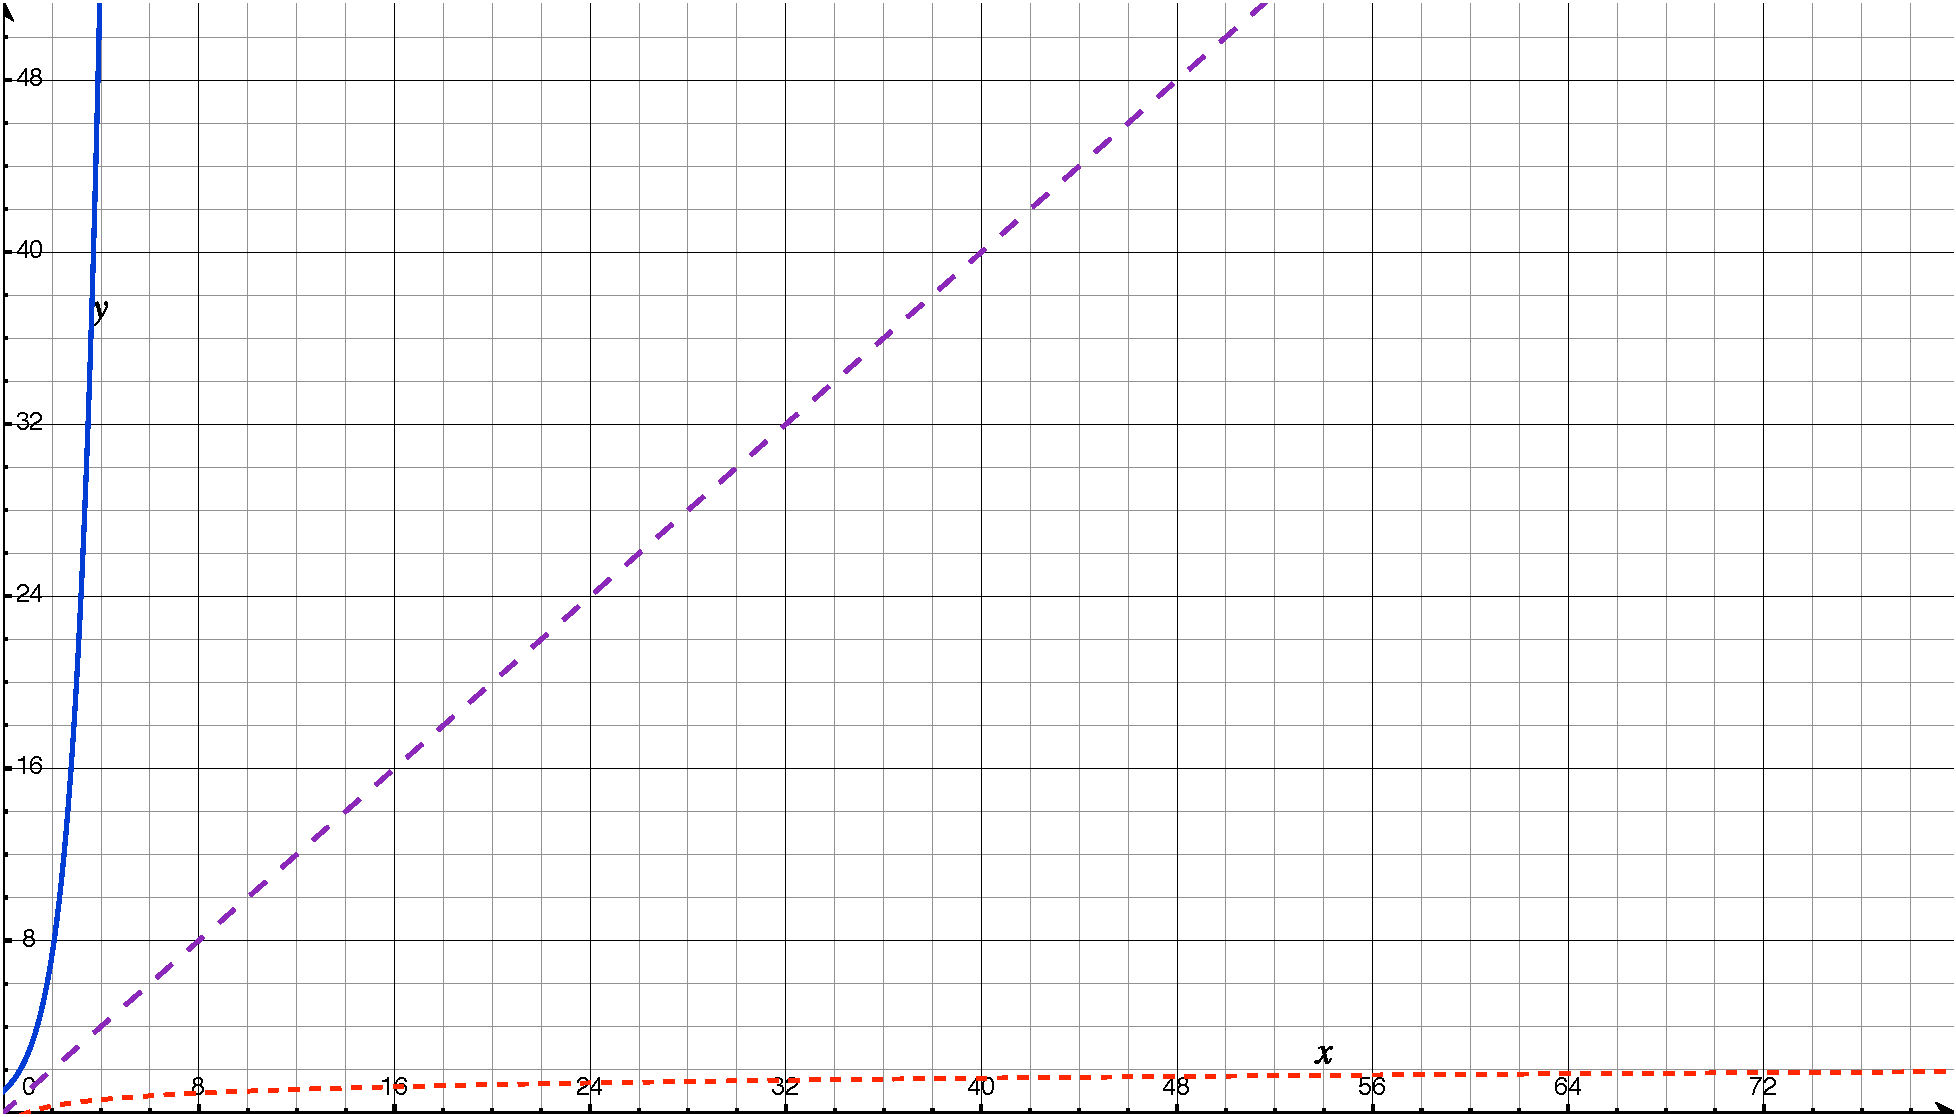
\includegraphics[width=0.8\textwidth]{Complexity.pdf}
\end{center}
As you can see,
except for very small sizes,
something with complexity $\mathcal{O}(\log n)$ is crazy fast compared 
to something with complexity $\mathcal{O}(n)$,
and for reasonably big problem sizes,
we might as well give up on any process with exponential complexity,
because we may never get the answer.
Unfortunately, many important problems do have exponentially complex solutions,
so computer scientists have found and continue to search for faster methods of
almost solving the problems.

Fortunately, the tree data structure leads naturally to algorithms with log complexity.
Let's figure out why, by looking at one of the nicest examples,
a balanced binary tree,
\begin{code}
type BTree a = Empty | Branch a (BTree a) (BTree a)
\end{code}
which, for simplicity, we populate with numbers,
\begin{code}
tree = Branch 10 (Branch 6  (Branch 3  (Branch 1 Empty Empty)
                                       (Branch 4 Empty Empty) )
                            (Branch 8  (Branch 7 Empty Empty)
                                       (Branch 9 Empty Empty) )
                 (Branch 17 (Branch 12 (Branch 11 Empty Empty)
                                       (Branch 14 Empty Empty) )
                            (Branch 25 (Branch 20 Empty Empty)
                                       (Branch 30 Empty Empty) )
\end{code}
which is easier to understand if drawn:
\[
\fbox{ \xygraph{
!{<0cm,0cm>;<1cm,0cm>:<0cm,1cm>::}
!{(1,0)}{1}="1"
!{(2,1)}{3}="3"
!{(3,0)}{4}="4"
!{(4,2)}{6}="6"
!{(5,0)}{7}="7"
!{(6,1)}{8}="8"
!{(7,0)}{9}="9"
!{(8,3)}{10}="10"
!{(9,0)}{11}="11"
!{(10,1)}{12}="12"
!{(11,0)}{14}="14"
!{(12,2)}{17}="17"
!{(13,0)}{20}="20"
!{(14,1)}{25}="25"
!{(15,0)}{30}="30"
"10":"6"
"10":"17"
"17":"25"
"17":"12"
"25":"30"
"25":"20"
"12":"14"
"12":"11"
"6":"8"
"8":"7"
"8":"9"
"6":"3"
"3":"1"
"3":"4"
}}
\]
It is a \emph{binary} tree because each node has two outgoing edges.
It is an \emph{ordered} binary tree because at every node, the subtree going left is labelled only by values less than the current value, and the subtree going to the right is labelled only by values greater than the current value.
It is a \emph{balanced} tree because from the head node, all of the maximal paths are the same length or close to it,
or said another way,
all of the lowest boughs touch the ground.

The great thing about a tree labelled in this way is that to test for membership in the set of node labels,
we can start at the top and test for ordering (being less than, equal, or greater than) once at each level, going down if the current node label is not what we are looking for.
At most we need as many comparisons as the tree is heigh.
Since the number of nodes is $1 + 2 + 4 +  2^{h-1} = 2^h - 1$,
where $h$ is the height of the tree, we conclude that
it takes $\mathcal{O}(\log_2 n)$ steps to test for membership
in a set when stored in a balanced binary tree.

Now, if we labelled the tree with a pair \texttt{(key,value)} of types, where the \texttt{key} type is used for looking up associated \texttt{value}s, we would have an $\mathcal{O}(\log_2 n)$ method of looking up associated values---just like a \texttt{Dict}!

If we stored our values
\begin{code}
asAList = [1,3,4,6,7,8,9,10,11,12,14,17,20,25,30]
\end{code}
on the other hand,
we would be stuck with linear complexity.

\medskip
The moral of the story is that it is well worth spending a few days to really learn the container types in ELM, 
and save a lot of time \emph{not} waiting for \texttt{Dict} lookups in the future.

%\chapter{Records and The ELM Architecutre}
%%
%We now have the basic ingredients for understanding
%the \emph{ELM Architecture},
%which is the preferred way of building ELM applications.
%There is no Interpol department assigned to enforce this, 
%but if you are going to read other people's code, 
%or want to share your own apps and components,
%it is good to stick to conventions.
%In fact, the ELM Architecture is really only making explicit the only sensible way to write user interfaces in ELM.
%
%Why now?  Because we needed the idea of state to capture the outside world first.
%The starting point for designing a UI is to 
%figure out what state the app must ``remember''
%and to which actions the app must respond.
%For really simple apps, the responses are uniform.
%Imagine, the Beep App has one action, clicking its single button,
%and it responds by beeping.
%But most apps respond differently to external actions
%depending on what state they are in.
%For example, asking to close a document when there are unsaved changes will---I hope---prompt for saving before losing changes.
%Making separate tables of state and user actions is only part of the story, 
%better to use a state diagram to capture all allowed sequences of user interaction.
%For even moderately interesting applications,
%this is not enough.
%Any app getting images from the internet,
%posting high scores to a leader board,
%or including animations
%will also need to respond to network or internally generated events for things like:  completion of a download, passage of time, or loss of network connectivity.
%
%As an aside, before we explain the ELM Architecture, why does software have \emph{architecture}?
%What is the relationship to design?
%Both words are borrowed from art and building,
%with design originating in the marking of the outlines of, e.g., a building, and architecture coming from the Greek word for builder.
%In software, architecture means either a framework of rules to be used in designing software, or it means the highest-level part of the design.
%For a beginner, the existence of two words for this process should be evidence that software design is not easy.
%More information, and a wealth of references is available at
%\url{https://en.wikipedia.org/wiki/Software_architecture}.  
%
%\emph{not finished!}

%-- now add controls for single paddle
%  - two kinds of events, so we need sum type
%  
%-- what if we want to add undo
%  -- what is reification
%  -- deep embedding, and shallow embedding
%  
%-- refer to ELM Architecture 
%  - sum type is called union type

\chapter{Algebraic Expressions}

Every language needs \emph{nouns} and \emph{verbs}.  
Things, and what happens to them.
In Computer Science, we have data, and functions.

In this module, we define a language of the types of algebraic expressions you use in Calculus.

\begin{code}
type Exprs = Const Float
           | Var String         -- in math we often use Char
           | Sqrt Exprs         -- we can take sqrt(anything)
           | IntPow Exprs Int   -- the easy case of exponent
           | Exp Exprs          -- e^expr
           | Ln Exprs
           | Mult Exprs Exprs
           | Add Exprs Exprs
           | Neg Exprs
\end{code}
To save ourselves some headaches later, we do not allow 
expressions like $x^y$, but restrict our expressions to 
integer powers $x^n$ where $n$ is an integer.
In mathematics, we usually use a single letter for a variable,
but then we also end up using subscripts, superscripts, greek and other 
alphabets and accents.
Since ELM \verb|String|s are made up of Unicode characters,
you can pretty much do any of those things, as long as you can
remember the keyboard tricks to type them all in.
I'll stick to English words, contracted and sometimes squished together.
We also need the \verb|Var| constructor, which signals that this particular \verb|String| is the name of a variable.
In pen-and-paper mathematics, we would never write something like that.
The same symbol can mean different things in different contexts.
We just need to remember which type of math we are doing.
This is even more clear for constants,
where $0$ could be a number zero, but it could also be a function which is always zero, or a vector which is zero.

Since this data type refers to itself in some of its constructors,
so we could call it a \emph{self-referential} data type.
In some programming languages, 
this is harder to do, but it is so easy to do in
ELM that it hardly gets mentioned.
It is, however, commonly called an \emph{algebraic} data type.
Either way, is the mirror-image of the Divide \& Conquer algorithms
and you can expect to see them here.

To make it easier to create examples, we predefine some variables 
\begin{code}
x = Var "x"
y = Var "y"
z = Var "z"
\end{code}
so you can refer to them without needing to repeatedly type \verb|Var|.
For example
\begin{code}
xXy =  Mult x y
\end{code}
You can now type in some of your favourite expressions
that bring back fond memories of High School math class.
Here are some of our favourites:
\vspace{-12pt}
\begin{code}
example = Add (Const 7) (Mult (Const 4) (Add (Sqrt x) (Exp y)) )
example2 = Add (Var "x") (Var "y")
example3 = Mult (Var "z") (Const 0)
example4 = Add (Sqrt (Mult (Var "x") (Const 0))) (Var "y")
example5 = (Sqrt ( (Const 0)))
example4Again = Add (example5) (Var "y")
\end{code}

\medskip
Once you've typed those in, I bet you have a hard time reading them.
The \verb|Exprs| language is just not as easy to read as the mathematical expressions we are used to,
but we can partially fix that by adding a function to 
translate \verb|Exprs| into a string of characters  which
look a lot like pencil-and-paper expressions.

Expressions can get long and complicated,
but we can always break them up into similar pieces,
and using Divide \& Conquer means that we only have to 
figure out the simplest possible expressions, and then
let the function do all the work:
\begin{code}
pretty : Exprs -> String
pretty e = case e of
            (Var name) -> name
            (Mult expr1 expr2) -> "(" ++ (pretty expr1) ++ ")" ++ " * " ++ "(" ++ (pretty expr2) ++ ")"
            (Sqrt expr) -> "sqrt(" ++ (pretty expr) ++ ")"
            (Const c) -> show c
            (IntPow expr exponent) -> "(" ++ (pretty expr) ++ ")^(" ++ (show exponent)++")"
            (Exp expr) -> "e^("++ (pretty expr) ++ ")"
            (Ln expr) -> "ln("++pretty expr++ ")"
            (Add expr1 expr2) -> (pretty expr1) ++ " + " ++ (pretty expr2)
            (Neg expr) -> "- (" ++ pretty expr ++ ")"
\end{code}

Since our constants are not real numbers, 
but floating point approximations,
we need to know a bit about the difference.
Floating-point numbers are like numbers in scientific notation,
they contain an exponent, and a fractional number with a fixed 
number of digits of precision.  
Of course, the exponent and fractional part are stored in binary
so the precision is measured in binary digits (\emph{i.e.}, bits)--%
of which a \verb|Float| has 53--%
and the maximum exponents are $2^{1023}$.
Irrational numbers like $\sqrt{2}$ and $\pi$ cannot be represented
exactly, but other numbers like $101$ and $2.5$ can.
In addition to ``normal'' numbers,
there are also special bit-patterns for $\infty$, $-\infty$
and \verb|NaN| (not-a-number).
These numbers follow a standard representation in bits created by
a committee of the IEEE (Institute of Electrical and Electronics Engineers).

Knowing that these are only approximations,
most people are not surprised that errors can build up when
real numbers are rounded-off to the best approximation,
but most people \emph{are surprised} that \verb|NaN| is not
equal to itself.
If you want your functions to work with \verb|Float|s,
you need to be aware of this.

The main advantage of using IEEE standard numbers is that you can
share your numbers with people using other computers.
The reason \verb|NaN| is useful,
is that you don't need to test for potential errors all over your code,
you can let just check the final result with 
\begin{verbatim}
isNaN : Float -> Bool
\end{verbatim}
because once a \verb|NaN| is generated, it will propagate through
the computation to the final result.
Adding, subtracting, taking an exponent, \emph{etc.} of a \verb|NaN|
produces another \verb|NaN|.
This is really important when we want to do a lot of calculations
in parallel to make things faster.
Since \verb|NaN|s propagate, all of our computations can work in parallel
which allows CPUs to process tens of operations at the same time, 
and GPUs to process many thousands all together.  
This is really useful in imaging when we have millions of pixels
all requiring the same calculations to render a scene or reconstruct a medical image.

\section{Simplification}

\begin{code}
simplify : Exprs -> Exprs
\end{code}
$x \cdot 0 \mapsto 0$  (commutative)
\vspace{-12pt}
\begin{code}
simplify e = case e of
               (Mult x (Const 0)) -> Const 0
               (Mult (Const 0) x) -> Const 0
\end{code}
$x^1 \mapsto x$
\vspace{-12pt}
\begin{code}
               (IntPow x 1) -> x
\end{code}
$x\cdot x \mapsto x^2$
Since we cannot match the same value twice in the Divide step,
we have to match x*y and add a condition that they be equal ( $x == y$).
\vspace{-12pt}
\begin{code}
               (Mult x y) -> case x == y of
                               True  -> IntPow x 2
                               False -> Mult (simplify x) (simplify y)
\end{code}
$x^n * x \mapsto x^{n+1}$
is complicated, because we cannot use $x$ twice on the LHS
\vspace{-12pt}
\begin{code}
               (Mult (IntPow x n) y)
                               -> case x == y of
                                    True -> IntPow x (n+1)
                                    False -> Mult (IntPow (simplify x) n) (simplify y)
\end{code}
$x + 0 \mapsto x  (commutative)$
\vspace{-12pt}
\begin{code}
               (Add x (Const 0)) -> x
               (Add (Const 0) x) -> x
\end{code}
$x * 1 \mapsto x  (commutative)$
\vspace{-12pt}
\begin{code}
               (Mult x (Const 1)) -> x
               (Mult (Const 1) x) -> x
\end{code}
$\sqrt{x^{2n}} \mapsto x^n$ \\
$\sqrt{x^{2n+1}} \mapsto x^n\sqrt x$ 
\vspace{-12pt}
\begin{code}
               (Sqrt  (IntPow x exponent))
                  -> case exponent % 2 of  -- remainder
                       0 -> IntPow x (exponent // 2)
                       _ -> Mult (IntPow x (exponent // 2)) (Sqrt x)
\end{code}
In the next rules, we check to see if an operation is applied to
a constant, in which case we can calculate the result right away,
because there are no variables involved.
$\sqrt{\text{\texttt{Const}}\, c} \mapsto \text{\texttt{Const}} \sqrt{c}$
\vspace{-12pt}
\begin{code}
               (Sqrt (Const c)) -> Const (sqrt c)
\end{code}
The same works for the other operations
\vspace{-12pt}
\begin{code}
               (Add (Const c1) (Const c2)) -> Const (c1 + c2)
               (IntPow (Const c) n) -> Const (c^n)
               (Exp (Const c)) -> Const (e^c)
               (Ln (Const c)) -> Const (logBase e c)
               (Neg (Const c)) -> Const (-c)
\end{code}
$\text{NaN} + x \mapsto \text{NaN}$  (this one is tricky)
\vspace{-12pt}
\begin{code}
               (Add (Const x) y)
                  -> case isNaN x of
                       True  -> Const x
                       False -> Add (Const x) (simplify y)
\end{code}
If none of the above patterns is matched, 
we have to look deeper in the expression tree to find something
to simplify.
This is the \emph{Divide} step!
Since there are multiple data constructors which contain 
subexpressions, we need multiple rules to implement the Divide step.
All of the rules are similar to
$e_1 * e_2 \mapsto \text{simplify}(e_1) * \text{simplify}(e_2)$
\vspace{-12pt}
\begin{code}
               (Mult expr1 expr2) -> Mult (simplify expr1) (simplify expr2)
\end{code}
but each handles a different outermost operation:
\vspace{-12pt}
\begin{code}
               (Add expr1 expr2) -> Add (simplify expr1) (simplify expr2)
               (Sqrt expr1) -> Sqrt (simplify expr1)
               (IntPow expr1 n) -> IntPow (simplify expr1) n
               (Exp expr1) -> Exp (simplify expr1)
               (Ln expr1) -> Ln (simplify expr1)
               (Neg expr1) -> Neg (simplify expr1)
               (Const c) -> Const c
               (Var name) -> Var name
\end{code}

Now each time we apply the \verb|simplify| function, it searches the 
expression tree for a pattern for which it has a rule, and applies 
that rule.  
Most expressions can be simplified by more than one rule,
and sometimes the second pattern we simplify is partially created by applying the first rule.
We need a way to keep applying rules until there are no more rules which apply.
The easy way to do this is to apply \verb|simplify| and
check to see if the new expression is the same
\begin{code}
simplifyUntilItStops x = let xNew = simplify x
                         in case xNew == x || isConstNaN x of
                              True  -> x
                              False -> simplify xNew
\end{code}
where we use a helper function which checks for a NaN input,
since NaN is defined to be not equal to anything, including itself!
\vspace{-12pt}
\begin{code}
isConstNaN x = case x of
                 (Const x) -> isNaN x
                 y         -> False
\end{code}

\section{Derivatives}

Derivation is an operation which turns a an expression defining a continuous funciton and produces a new expression defining the slope of the tangent to the function at each point.
We call this the derivative.
In ELM, we everything we \emph{do} is a function, and we can translate the last sentence into this type
\vspace{-12pt}
\begin{code}
deriv : String {- variable with respect to which we take the derivative -}
      -> Exprs 
      -> Exprs
\end{code}
adding in the fact that we take the derivative with respect to a particular variable (which is defined by a string)--%
this is something we may expect a person to assume.

We define the function by encoding all the basic rules about derivatives one case at a time.
If the funciton is constant, of course, the slope is zero:
\vspace{-12pt}
\begin{code}
deriv varName e
  = case e of
      (Const c) -> Const 0
\end{code}
for example
$d/dx (x) = 1$ and   $d/dx (u) = 0$ (as long as $u$ is not the variable with respect to which we are taking the derivative.

A variable, on the other hand, has derivative $1$ if it is the right variable:
\vspace{-12pt}
\begin{code}
      (Var name) -> case varName == name of
                      True  -> Const 1
                      False -> Const 0
\end{code}
and the derivative of a sum is the sum of the derivatives:
\vspace{-12pt}
\begin{code}
      (Add e1 e2) -> Add (deriv varName e1) (deriv varName e2)
\end{code}
Did you notice Divide \& Conquer being applied in the last rule?  
The remaining rules will also implement D \& C,
but the combine steps get more complicated.

Let's start with the product rule:
\vspace{-12pt}
\begin{code}
      (Mult e1 e2) -> Add (Mult (deriv varName e1) e2) 
                          (Mult e1 (deriv varName e2))
\end{code}
The remaining cases are rules which are familiar from Calculus,
and some of them we call the Chain Rule.
\vspace{-12pt}
\begin{code}
      (Neg e1) -> Neg (deriv varName e1)
      (Sqrt e1) -> Mult (Const 0.5) (Mult (IntPow (Sqrt e1) (-1))
                                          (deriv varName e1)
                                    )
\end{code}
where, to see the application of the chain rule, we could write
$f(x)$ for \verb|e1| and $f'(x)$ for \verb|deriv varName e1|:
$$ \frac{\partial}{\partial x} \sqrt{f(x)} = \frac12 \frac{1}{\sqrt{f(x)}} f'(x).$$ 
\vspace{-12pt}
\begin{code}
      (IntPow e1 n) ->  Mult (Mult (Const (toFloat n)) (IntPow e1 (n-1)))
                             (deriv varName e1)
      (Exp e1) -> Mult (deriv varName e1) (Exp e1)
      (Ln e1) -> Mult (IntPow e1 (-1))
                      (deriv varName e1)
\end{code}

\chapter{Say Goodbye to Mediocre Presentations, and Closed Types}
%
As a growing ELM programmer you have probably noticed your enjoyment of life goes up as your brainpower expands,
but even as your life gets better, 
there is a dark force eroding the foundations of the space-time continuum.
Listen carefully, and you may be able to 
Yes, I am --speaking-- writing out-loud about hear the droning from boardrooms across the planet caused by needlessly mediocre slide presentations.

\medskip
Be part of the solution!  Write your presentations in ELM!

\medskip
To get you started, I've created a template for a slide presentation,
in which arrow keys advance (and retreat) through your slides,
and each slide has an animation, which restarts whenever you come back to a slide.
To make this work, we need to get \texttt{Signal}s generated when arrow keys are pressed,
and to animate the slides, we need a time signal.
Since there are two types of \texttt{Signal}s we respond to,
we need to bring them together in a union type
\begin{code}
type Events = Arrows {x : Int, y:Int} 
            | TimeIncrease Float
\end{code}
which captures the types of \texttt{Signal}s we process,
and a we merge the two streams of \texttt{Signal}s with a function mysteriously called \texttt{merge}
\begin{code}
events : Signal Events
events =
   Signal.merge
       (Signal.map Arrows       Keyboard.arrows)
       (Signal.map TimeIncrease (fps 40))
\end{code}
In addition to recording the cause of the latest signal, so we can do the right thing,
the \texttt{Event} type solves a typing problem for us, namely, 
the fact that \texttt{Keyboard.arrows} and \texttt{fps 40} have different types.
Since they have different types, we cannot put them in an ELM \texttt{List},
 unlike English lists which allow mixed categories and even parts of speech in one lists---cows, pontificate, nicely\footnote{Duck your head while contrarians pounce on this one: since all of these are \emph{words}, they do form a homogeneous list.  But I think you know what I mean, and helps explain why English is a terrible language in which to program computers!}.

main =
 Signal.map view <| Signal.foldp update (0,1) events

-- the update has to handle both types of signals
update event (t,idx)
 = case event of
     -- if an arrow is pressed, move to another slide, and reset time
     Arrows arrows   -> (0     , moveIdx arrows idx)
     -- if time goes by, update the time in the state (for animations)
     TimeIncrease dt -> (t + 0.001 * dt, idx)

-- to avoid going past the first/last slides, check before changing 
-- the slide index
moveIdx arrows oldIdx = case arrows.x of
                        1  -> if oldIdx + 1 < Array.length slides 
                              then oldIdx + 1
                              else oldIdx
                        (-1) -> if oldIdx > 0
                              then oldIdx - 1
                              else oldIdx
                        otherwise -> oldIdx

-- even though we cannot go past the last slide,
-- we need to check that the slide lookup in the array of slides works
-- and display a blank collage if we are out of range
view (t,idx) = case Array.get idx slides of
                Just slide -> slide t
                Nothing    -> collage 400 400 []

-- the list of slides is stored in an array (because this is O(1) lookup)
slides = Array.fromList [slide1,slide2,slide3]

slide1 t = collage 400 400 [filled blue (circle 10) |> move (100*sin t,0)]

slide2 t = collage 400 400 [filled purple (circle 10) |> move (100*sin t,0)]

slide3 t = collage 400 400 [filled red (circle 10) |> move (100*sin t,0)]

\chapter{Wires \& Switches}
%
{\textit{
Do you remember a time when your parents thought you were sleeping, but you were really making secret plans via flashlight signals with your accomplice?
You were encoding information by turning the flashlight \emph{ON} and \emph{OFF} (or maybe by using long and short flashes).}
\bigskip

Inside every iPad or smartphone is a computer crammed with billions of wires, tiny versions of the wires connecting a flashlight's battery and light, and all the pictures, texts, and numbers you put into that device are encoded into groups of \emph{ON} and \emph{OFF} states.

Every spelling mistake you fix or sketch you make happens by flipping switches.

How can we do all that with \emph{ON} and \emph{OFF}?  Well, first of all, we have billions of switches in here, and we are very organized!

To start, let's agree that \emph{ON} will mean 1 and \emph{OFF} 0.  
Just as with normal decimal numbers, we can group these bits (short for binary digits, \emph{bi} meaning two) to make bigger numbers.
Counting in binary:
\begin{center}
\begin{tabular}{rcccccccc}
decimal & 0 & 1 & 2 & 3 & 4 & 5 & 6 & $\cdots$\\
binary & 0 & 1 & 10 & 11 & 100 & 101 & 110 & $\cdots$\\
\end{tabular}
\end{center}
You get the idea!

Starting with something as simple as \emph{on/off},
we have built up a system of numbers.
Letters are easy, just number them 1 for A, 2 for B, 
and so on, and we can encode text.
If you write fancy text,
you will need Unicode\footnote{\url{http://www.unicode.org}},
which is an agreed encoding of any symbol you are likely to need,
and even of symbols for the undeciphered Linear~A script of Minoa (ancient Greece),
and---just in case you find a recipe to turn dust into gold---mediaeval alchemical symbols.

Images are also easy to encode. 
Chop them into little squares, and encode the intensity of the primary colours in each square as a number.
If you really are reading this on an iPad,
you can try this out with our \emph{free} app Image~2~Bits,
 for black~=~1 and white~=~0 images.

One thing I cannot explain is why all of our technology based on \emph{binary} encoding is called \emph{digital}\footnote{Wikipedia blames it on 
the mathematician George Stibitz.}!

\section{CPU}
%
So encoding information as on/off choices is not hard,
but how do we process that information?
While decoding images and text can be a interesting mental exercise,
the real advantage of the information revolution is not just the better storage of information,
but the ability of computing machinery to process it for us.
Think about it, even looking something up on the internet involves many computers processing that information.
The computer at the source needs to separate the information you want from all the other information,
then it needs to find a path through the web of the internet to send that information back to your computer,
then your computer needs to make the answer visible or audible to you.
Ok, now you can ask the internet ``Are there really butterflies in my stomach?''  and all your other pressing questions.

\medskip
What puts the ``automatic'' in automatic data processing is the ability of the billions of switches in our favourite information appliances to turn on and off in response to other switches,
and by really cleverly connecting those switches together with tiny wires.
Every year, those switches and wires are made even smaller,
so that today you could not even see the individual switches with a microscope.  
Normal light is just too ``big'' to see them.
This helps in two ways:
smaller switches using less material are cheaper,
and information gets around faster ask distances shrink,
since all information has to obey one speed limit---the speed of light\footnote{There is actually a method of appearing to send information faster than light using the separation of particles coupled by quantum mechanical mechanisms,
but only by spending even longer to separate the particles in the first place.}. 

Realistically, I'm going to need to skip some steps in order to explain how a billion switches are organized into a CPU.
So rather than building up complexity step by step,
let's use an approach which works for developers of business software: model the data and then the processes.
A difficult client may not be able to tell you what the data is,
and when they explain the processes involved, 
they will skip a bunch,
but if you cannot put these two things down on paper, 
you better hope you are getting paid by the hour and not for finishing the job.

So what is the data we need to worry about.
If you know something about what science has uncovered about the processor you carry around in your head,
you  know that everyone has a measurable ability to juggle a small number of facts at once.
This is called \emph{short term memory},
and for most people it is about seven numbers, 
and although you can improve it with training,
it will not change by much.
On the other hand, even small changes can have big impacts on how 
good you are at logical thinking---solving logic puzzles and math problems.
Once you get past that small number of facts you can juggle,
you need another mechanism.
Most of us were taught to write out all the facts in a problem before trying to solve it.
This ``outsources'' the juggling problem to a piece of paper,
and it is even more effective if you can create some kind of diagram to connect your data together.
This is exactly why state diagrams are so useful 
in helping us design complex software, 
or helping us make sure what we implement really does what it is supposed to do.

Why do we have such a small working memory?
Well, I am not an expert in evolutionary biology,
but if you accept the fact that our brain uses 
energy and oxygen\footnote{Actually, the brain uses more than its share of oxygen by weight, about a quarter of your body's supply, which is physical training is a good way to boost your capacity to write exams or get complicated ELM programs to work.}
and taking things to the limit,
a very smart human who did not have much energy left for running
probably would not have survived very long in the African savannah,
so it is clear that there was evolutionary pressure not to make the brain \emph{too} big.
On the other hand,
remembering that our cousins who decided to live in caves with tigers do not come to our birthday party any more,
and being able to conclude that keeping a distance from known tiger haunts would keep us alive.
So clearly there is a good balance there.
The really amazing thing is that the evolutionary pressures of a million years ago produced a brain which can survive in the information age.

\medskip
In a \emph{central processing unit}, a CPU,
there is also a trade-off, but for registers,
which are the CPUs version of working memory,
the trade-off is in speed and cost but not energy. 
To organize billions of \emph{dynamic} switches,
we organize them in cascading networks,
which we can imagine as inputs starting at the 
top and feeding the first row of switches,
whose outputs feed the second row of switches,
and so on.
So that they can do more than one computation,
once the first row of switches has changed in response to its inputs, a second set of inputs can be processed.
This is similar to how the \texttt{foldp} function applies a function to a list of signal inputs and the current state.
In this case, the current state would be the output of the row of switches, 
and dependence on the current state would be implemented as wires which loop from the outputs back to the inputs.
Although we did not need to chain together multiple \texttt{foldp},
you could imagine that more complicated programs may need to do so.
Since the basic building block of computation is a simple switch,
we cannot really do anything without many rows,
which would be the equivalent of many \texttt{foldp}s chained together.

In our ELM programs, new signals came from user interaction or timers set to create signals, like \texttt{fps}, which creates signals a number of times every second.
In the CPU, so that in inputs do not arrive before the outputs are ready,
each row of switches is separated from the previous one by a special row of switches called \emph{latches} because they latch onto an output of the previous row, and maintain it as the input of the next row until a secondary signal causes them to drop the old value and pick up new input values.
The trick of designing high performance CPUs is to create switch geometries such that the slowest switch anywhere in the CPU is as fast as possible.
Once this time is known, a signal which turns on and off at this speed is provided as an input to every latch in the CPU, 
and 0 and 1 values will march from row to row at the rate of this signal.
This is what is called the clock rate, and currently measured in gigahertz (GHz), meaning that 0s and 1s march through each row several billion times per second.

\medskip
At this point, is challenging, but possible, to design the main components of a CPU,
what we call ALUs, \emph{arithmetic logic units},
which take rows of inputs representing binary numbers or lists of bits, and after a few or a few 10s of rows, output the addition or multiplication of the inputs as binary numbers, or perform logical operations on the individual binary digits (bits).
To keep things moving, we need to quickly retrieve inputs and store outputs to short-term memory.
Since electrical signals can at most travel as fast as the speed of light,
larger short-term memories, requiring more switches, and therefore more area on the CPU lead to larger wires, and slower retrieval and storage.
It turns out that seven is also about how many registers were found to make efficient CPUs, with the earliest CPUs having only a few, and for a long time most CPUs having eight registers.
It is only relatively recently that more complicated CPU designs have made it practical to have much larger numbers of registers (32,64, or even 128).

Just as people used pencil and paper, and library books to store a larger number of facts before the age of computing machinery,
the CPU has the capacity to store more facts than fit in working memory, 
and in the CPU these are mostly stored as RAM (random access memory) and on hard drives\footnote{Actually, much of the performance improvements in recent years have come from new classes of memory which change the trade-off between speed and cost.}.

\medskip
So to get back to our model of data in the CPU
we will stick to eight registers (containing integers
\begin{code}
type alias RegisterValue = Int
\end{code}                          
) which gives us a data model
\begin{code}
type CPUState = CPUState  ( RegisterValue, RegisterValue
                          , RegisterValue, RegisterValue
                          , RegisterValue, RegisterValue
                          , RegisterValue, RegisterValue)
\end{code}
Which would be enough if our CPUs did the same computation over and over,
but unlike a cement mixer, which can only mix cement (or perhaps dough for the worlds largest pizza),
CPUs are so valuable because they can do any computation we can think of.
To handle this, we need to be able to \emph{program} them,
we we do by giving them a list of instructions.
Think of it as a task list,
which is not useful if you do not track completed tasks.
We do this by adding
\begin{code}
                          CurrentInstruction
\end{code}
(another type alias for \texttt{Int})
to the data model.
But with such a model,
we would still need to write a different program for each set of possibilities in a program, since there is only one list.
If, however, we had the possibility to make tests of the current state and jump around in the list of instructions,
we can have one program which can write personalized birthday invitations to our friends and address each of them in their native language.
To handle the jumping, we add the result of the last comparison. 
\begin{code}
                          ComparisonResult
\end{code}
And, finally, assuming there is a finally for our program,
we need 
\begin{code}
                          (Maybe HaltedBecause)
\end{code}
to indicate whether the CPU has reached the end of the program,
stopped because there was an error, 
\begin{code}
type HaltedBecause  = ReachedHalt
                    | IllegalRegisterNum
                    | IllegalAddress
                    | IllegalInstrAddress
\end{code}
or, in the case of \texttt{Nothing}, is still running our program.

Our processor will only make simple numerical comparisons,
which we can model with ELM's \texttt{Order} type
\begin{code}
type alias ComparisonResult = Order
\end{code}

\medskip
Next, in the language of business\footnote{People in business don't like that name, so they call it Enterprise Software.} software development,
we need to list the processes.
We can list them from the software point of view as
\emph{instructions}
\begin{code}
type Instruction  = Load           RegisterNumber RegisterNumber RegisterNumber
\end{code}
is an instruction to move a value from main memory to a register.  
By convention, the first listed register number is the destination, and the address is the sum of the second two register values.  If the address does not exist, the processor must halt with an error.
\begin{code}
                  | Store          RegisterNumber RegisterNumber RegisterNumber
\end{code}
is an instruction to move a value from a register to main memory.
By convention, the first listed register number is the source register, and the destination address is the sum of the second two register values.  If the address does not exist, the processor must halt with an error.
\begin{code}
                  | LoadImmediate  RegisterNumber RegisterValue
\end{code}
Sometimes, a value is always the same, so we don't need to bother putting it in main memory,
we have this special instruction to load the value contained in the instruction.
\begin{code}
                  | Add            RegisterNumber RegisterNumber RegisterNumber
\end{code}
This is the first instruction which calculates a new value, in this case, and addition of integers.
By convention, the first listed register number is the destination, and the values in the second two registers are added.
\begin{code}
                  | Multiply       RegisterNumber RegisterNumber RegisterNumber
\end{code}
Similarly, the first listed register number is the destination, and the values in the second two registers are multiplied.
\begin{code}
                  | And            RegisterNumber RegisterNumber RegisterNumber
                  | Or             RegisterNumber RegisterNumber RegisterNumber
\end{code}
As with add and multiply, and and or take two inputs and put an output back in the first register,
but instead of treating the bits in the register a number, they treat them as a bunch of bits and perform logical operations on each of the bits.  For example
\begin{center}
\begin{tabular}{rcccc}
   & 0 & 0 & 1 & 1 \\
\texttt{And} & 0 & 1 & 0 & 1 \\ \hline
= & 0 & 0 & 0 & 1
\end{tabular} 
\quad and \quad
\begin{tabular}{rcccc}
   & 0 & 0 & 1 & 1 \\
\texttt{Or} & 0 & 1 & 0 & 1 \\ \hline
 = & 0 & 1 & 1 & 1
\end{tabular}
\end{center}
shows the results of \texttt{And}ing and \texttt{Or}ing 4-bit numbers, although our \texttt{RegisterValue}s are 32-bits wide.
\begin{code}
                  | Not            RegisterNumber RegisterNumber
\end{code}
\texttt{Not} reverses the bits.
\begin{center}
\begin{tabular}{rcccc}
\texttt{Not} & 0 & 1 & 0 & 1 \\ \hline
 = & 1 & 0 & 1 & 0
\end{tabular}
\end{center}
\begin{code}
                  | Rotate         RegisterNumber RegisterNumber Int           
\end{code}
while \texttt{Rotate} spins them around to the right, 
$$
00001000 \overset{rotate\ 1}{\longrightarrow} 00000100, \quad 
11000000 \overset{rotate\ 6}{\longrightarrow} 00000011,\quad 
00000001 \overset{rotate\ 1}{\longrightarrow} 10000000,
$$
putting them back in on the left when they fall off the end.  (Again shown with shorter 8-bit numbers rather than the normal 32-bits.)

Doing different things depending on input data, or different user actions is accomplished
at the CPU level by being able to compare numbers and then jump to a different instruction in the the machine program rather than continuing, only if the conditions are true. 
\begin{code}
                  | Compare        RegisterNumber RegisterNumber
\end{code}
does the comparisons of two register values, and puts the result of the compare into the \texttt{CPUState}.
\begin{code}
                  | Branch         (List ComparisonResult) RegisterNumber
\end{code}
optionally jumps to an instruction number given by the specified register if the current condition in the \texttt{CPUState} is in the \texttt{List} of \texttt{ComparisonResult}s.

And finally, when our program is really finished, we can save electricity and turn our CPU off with the \texttt{Halt} instruction.
\begin{code}
                  | Halt
\end{code}
For safety, there should always be a \texttt{Halt} at the end of the list of instructions, even if the CPU will never get there because of \texttt{Branch}es.  In particular, if all the conditions are listed, the CPU will always jump to the indicated location in the program!

\section{Traces}
%
Just like an accident investigator for the Transportation Safety Board,
if something goes wrong with a machine program, 
we need to retrace the steps which led to the illegal instruction or incorrect result.
For the simplified CPU we are studying, 
all we need to know are the initial CPU state and memory state and the program,
because our CPU is \emph{deterministic}---it will always arrive at the same result when starting with the same inputs\footnote{If you are an aficionado of computer games, you may be puzzled by the apparent random events which happen in your games!  Even on deterministic CPUs, we can fake randomness by using some data which changes as an input.  For a game, the start time of the game, measured in seconds from 1970, is generally random enough, but for more serious matters, like choosing random seeds to encrypt our secret messages, most CPUs have even better ways of generating random numbers.}.

\medskip
Given the program,
\begin{verbatim}
number  instruction
 (0,  LoadImmediate 7 2),  
 (1,  LoadImmediate 2 1),  
 (2,  LoadImmediate 3 3),  
 (3,  LoadImmediate 4 (-1)), 
 (4,  LoadImmediate 5 16),    
 (5,  LoadImmediate 6 6),    
 (6,  Multiply 2 7 2),
 (7,  Compare 2 5),
 (8,  Branch [LT] 6),
 (9,  Halt)
\end{verbatim}
we can write out the state of the CPU at each instruction, and obtain a \emph{program trace}: \\
\noindent
\!\!\!\begin{tabular}{|p{0.04\textwidth}|p{0.07\textwidth}|p{0.07\textwidth}|p{0.07\textwidth}|p{0.07\textwidth}|p{0.07\textwidth}|p{0.07\textwidth}|p{0.07\textwidth}|p{0.07\textwidth}|p{0.07\textwidth}|p{0.07\textwidth}|}
\hline
clock time & current {\tiny instructn} & Reg 1 & Reg 2 & Reg 3 & Reg 4 & Reg 5 & Reg 6 & Reg 7 & Reg 8 & {\scriptsize Condition} \\
\hline
1 & 0 & 0 & 0 & 0 & 0 & 0 & 0 & 0 & 0 & EQ \\ \hline
2 & 1 & 0 & 0 & 0 & 0 & 0 & 0 & 2 & 0 & EQ \\ \hline
3 & 2 & 0 & 1 & 0 & 0 & 0 & 0 & 2 & 0 & EQ \\ \hline
4 & 3 & 0 & 1 & 3 & 0 & 0 & 0 & 2 & 0 & EQ \\ \hline
5 & 4 & 0 & 1 & 3 & -1 & 0 & 0 & 2 & 0 & EQ \\ \hline
6 & 5 & 0 & 1 & 3 & -1 & 16 & 0 & 2 & 0 & EQ \\ \hline
7 & 6 & 0 & 1 & 3 & -1 & 16 & 6 & 2 & 0 & EQ \\ \hline
8 & 7 & 0 & 2 & 3 & -1 & 16 & 6 & 2 & 0 & EQ \\ \hline
9 & 8 & 0 & 2 & 3 & -1 & 16 & 6 & 2 & 0 & LT \\ \hline
10 & 6 & 0 & 2 & 3 & -1 & 16 & 6 & 2 & 0 & LT \\ \hline
11 & 7 & 0 & 4 & 3 & -1 & 16 & 6 & 2 & 0 & LT \\ \hline
12 & 8 & 0 & 4 & 3 & -1 & 16 & 6 & 2 & 0 & LT \\ \hline
13 & 6 & 0 & 4 & 3 & -1 & 16 & 6 & 2 & 0 & LT \\ \hline
14 & 7 & 0 & 8 & 3 & -1 & 16 & 6 & 2 & 0 & LT \\ \hline
15 & 8 & 0 & 8 & 3 & -1 & 16 & 6 & 2 & 0 & LT \\ \hline
16 & 6 & 0 & 8 & 3 & -1 & 16 & 6 & 2 & 0 & LT \\ \hline
17 & 7 & 0 & 16 & 3 & -1 & 16 & 6 & 2 & 0 & LT \\ \hline
18 & 8 & 0 & 16 & 3 & -1 & 16 & 6 & 2 & 0 & EQ \\ \hline
19 & 9 & 0 & 16 & 3 & -1 & 16 & 6 & 2 & 0 & EQ \\ \hline
\end{tabular}\marginpar{$\frac{}{10}$}
\vspace{1mm}

\medskip
Creating a trace is a good way of checking your intuition about what a program does.
It is also recommended, along with two sudokus and ten servings of vegetables and fruit as part of your daily diet,
and is a favourite question to put on tests and exams, 
because it really tests your knowledge of the CPU state and transition functions---and it takes a while to fill out, giving the teacher a time for a nap.
Unless you happen to be an artificial intelligence, 
and you are labouring with the limitations of the human brain, 
including the tendency to get bored or complacent and make silly mistakes,
this is a good question to double check!





\end{document}
